% Template LaTeX file for DAFx-20 papers
%
% To generate the correct references using BibTeX, run
%     latex, bibtex, latex, latex
% modified...
% - from DAFx-00 to DAFx-02 by Florian Keiler, 2002-07-08
% - from DAFx-03 to DAFx-04 by Gianpaolo Evangelista, 2004-02-07 
% - from DAFx-05 to DAFx-06 by Vincent Verfaille, 2006-02-05
% - from DAFx-06 to DAFx-07 by Vincent Verfaille, 2007-01-05
%                          and Sylvain Marchand, 2007-01-31
% - from DAFx-07 to DAFx-08 by Henri Penttinen, 2007-12-12
%                          and Jyri Pakarinen 2008-01-28
% - from DAFx-08 to DAFx-09 by Giorgio Prandi, Fabio Antonacci 2008-10-03
% - from DAFx-09 to DAFx-10 by Hannes Pomberger 2010-02-01
% - from DAFx-10 to DAFx-12 by Jez Wells 2011
% - from DAFx-12 to DAFx-14 by Sascha Disch 2013
% - from DAFx-15 to DAFx-16 by Pavel Rajmic 2015
% - from DAFx-16 to DAFx-17 by Brian Hamilton 2016
% - from DAFx-17 to DAFx-18 by Annibal Ferreira and Matthew Davies 2017
% - from DAFx-18 to DAFx-19 by Dave Moffat 2019
% - from DAFx-19 to DAFx-20 by Gianpaolo Evangelista 2019
%
% Template with hyper-references (links) active after conversion to pdf
% (with the distiller) or if compiled with pdflatex.
%
% 20060205: added package 'hypcap' to correct hyperlinks to figures and tables
%                      use of \papertitle and \paperauthorA, etc for same title in PDF and Metadata
% 20190205: Package 'hypcap' removed, and replaced with 'caption', to allow for the inclusion
%			of a CC UP licence.
%
% 1) Please compile using latex or pdflatex.
% 2) If using pdflatex, you need your figures in a file format other than eps! e.g. png or jpg is working
% 3) Please use "paperftitle" and "pdfauthor" definitions below

%------------------------------------------------------------------------------------------
%  !  !  !  !  !  !  !  !  !  !  !  ! user defined variables  !  !  !  !  !  !  !  !  !  !  !  !  !  !
% Please use the following commands to define title and author(s) of the paper.
% paperauthorA MUST be the the first author of the paper
% Please comment the unused definitions 
\def\papertitle{Flexible real-time late reverberation synthesis with accurate parameter control}
\def\paperauthorA{Karolina Prawda}
\def\paperauthorB{Vesa V\"alim\"aki}
\def\paperauthorC{Silvin Willemsen}
\def\paperauthorD{Stefania Serafin}
% \def\paperauthorC{Author Three}
% \def\paperauthorD{Author Four}
%\def\paperauthorE{Author Five}
%\def\paperauthorF{Author Six}
%\def\paperauthorG{Author Seven}
%\def\paperauthorH{Author Eight}
%\def\paperauthorI{Author Nine}
%\def\paperauthorJ{Author Ten}

% Authors' affiliations have to be set below

%------------------------------------------------------------------------------------------
\documentclass[twoside,a4paper]{article}
\usepackage{etoolbox}
\usepackage{dafx_20}
\usepackage{amsmath,amssymb,amsfonts,amsthm}
\usepackage{euscript}
%\usepackage[latin1]{inputenc}
\usepackage[T1]{fontenc}
\usepackage[utf8]{inputenc}
%\usepackage[T1]{fontenc}
%\usepackage{lmodern}
\usepackage{nimbusserif}
\usepackage{ifpdf}
\usepackage[english]{babel}
\usepackage{caption}
\usepackage{subfig} % or can use subcaption package
\usepackage{color}
\usepackage{fancyref}
\usepackage{dirtytalk}
\usepackage{multirow}

\usepackage{caption}

\usepackage{subfig}

\usepackage[dvipsnames]{xcolor}
\newcommand{\silvin}[1]{\textcolor{ForestGreen}{#1}}
\newcommand{\karolina}[1]{\textcolor{blue}{#1}}
\newcommand{\vesa}[1]{\textcolor{red}{Vesa: #1}}
\newcommand{\stefania}[1]{\textcolor{Plum}{Stefania: #1}}


%\usepackage{dirtytalk}

\input glyphtounicode
\pdfgentounicode=1

\setcounter{page}{1}
\ninept

% build the list of authors and set the flag \multipleauth to handle the et al. in the copyright note (in DAFx_20.sty)
%==============================DO NOT MODIFY =======================================
\newcounter{numauth}\setcounter{numauth}{1}
\newcounter{listcnt}\setcounter{listcnt}{1}
\newcommand\authcnt[1]{\ifdefined#1 \stepcounter{numauth} \fi}

\newcommand\addauth[1]{
\ifdefined#1 
\stepcounter{listcnt}
\ifnum \value{listcnt}<\value{numauth}
\appto\authorslist{, #1}
\else
\appto\authorslist{~and~#1}
\fi
\fi}
%======DO NOT MODIFY UNLESS YOUR PAPER HAS MORE THAN 10 AUTHORS========================
%==we count the authors defined at the beginning of the file (paperauthorA is mandatory and already accounted for)
\authcnt{\paperauthorB}
\authcnt{\paperauthorC}
\authcnt{\paperauthorD}
\authcnt{\paperauthorE}
\authcnt{\paperauthorF}
\authcnt{\paperauthorG}
\authcnt{\paperauthorH}
\authcnt{\paperauthorI}
\authcnt{\paperauthorJ}
%==we create a list of authors for pdf tagging, for example: paperauthorA, paperauthorB, ... and paperauthorF (last author)
\def\authorslist{\paperauthorA}
\addauth{\paperauthorB}
\addauth{\paperauthorC}
\addauth{\paperauthorD}
\addauth{\paperauthorE}
\addauth{\paperauthorF}
\addauth{\paperauthorG}
\addauth{\paperauthorH}
\addauth{\paperauthorI}
\addauth{\paperauthorJ}
%====================================================================================

\usepackage{times}
% Saves a lot of ouptut space in PDF... after conversion with the distiller
% Delete if you cannot get PS fonts working on your system.


% pdf-tex settings: detect automatically if run by latex or pdflatex
\newif\ifpdf
\ifx\pdfoutput\relax
\else
   \ifcase\pdfoutput
      \pdffalse
   \else
      \pdftrue
\fi

\ifpdf % compiling with pdflatex
  \usepackage[pdftex,
    pdftitle={\papertitle},
    pdfauthor={\authorslist},
    pdfsubject={Proceedings of the 23rd International Conference on Digital Audio Effects (DAFx-20)},
    colorlinks=false, % links are activated as color boxes instead of color text
    bookmarksnumbered, % use section numbers with bookmarks
    pdfstartview=XYZ % start with zoom=100% instead of full screen; especially useful if working with a big screen :-)
  ]{hyperref}
  \pdfcompresslevel=9
  \usepackage[pdftex]{graphicx}
 % \usepackage[figure,table]{hypcap}
\else % compiling with latex
  \usepackage[dvips]{epsfig,graphicx}
  \usepackage[dvips,
    pdftitle={\papertitle},
    pdfauthor={\authorslist},
    pdfsubject={Proceedings of the 23rd International Conference on Digital Audio Effects (DAFx-20)},
    colorlinks=false, % no color links
    bookmarksnumbered, % use section numbers with bookmarks
    pdfstartview=XYZ % start with zoom=100% instead of full screen
  ]{hyperref}
  % hyperrefs are active in the pdf file after conversion
  %\usepackage[figure,table]{hypcap}
\fi
\usepackage[hypcap=true]{caption}
\title{\papertitle}

%-------------SINGLE-AFFILIATION SINGLE-AUTHOR HEADER STARTS (uncomment below if your paper has a single author)----------------------------------------
%\affiliation{
%\paperauthorA\,\sthanks{Thanks to the predecessors for the templates}}
%{\href{https://www.mdw.ac.at/ike/}{Institute 1} \\ University of Music and Performing Arts\\ Vienna, Austria\\
%{\tt \href{mailto:dafx2020@gmail.com}{dafx2020@gmail.com}}
%}
%-------------SINGLE-AFFILIATION SINGLE-AUTHOR HEADER ENDS-------------------------------------------------------------------------------------------------------------------

%------------SINGLE-AFFILIATION MULTIPLE-AUTHORS HEADER STARTS (uncomment below if your paper has two or more authors from the same institution)
%\affiliation{
%\paperauthorA\,\sthanks{Thanks to the predecessors for the templates}and \paperauthorB \,\sthanks{This work was supported by the XYZ Foundation}}
%{\href{https://www.mdw.ac.at/ike/}{Institute 1} \\ University of Music and Performing Arts\\ Vienna, Austria\\
%{\tt \href{mailto:dafx2020@gmail.com}{dafx2020@gmail.com}}
%}
%-----------------------------------SINGLE-AFFILIATION-MULTIPLE-AUTHORS HEADER ENDS----------------------------------------------------------------------------------------

%---------------TWO-AFFILIATIONS HEADER STARTS (uncomment below if your paper has two authors, each from a different institution)-----------------------------
\threeaffiliations{
\paperauthorA \,\sthanks{This work was supported by the "Nordic Sound and Music Computing Network---NordicSMC", NordForsk project number 86892.}}
{\href{https://www.aalto.fi/en/aalto-acoustics-lab}{Acoustics Lab} \\ Dept. of Signal Processing and Acoustics\\ Aalto University, Espoo, Finland\\
{\tt \href{mailto:karolina.prawda@aalto.fi}{karolina.prawda@aalto.fi}}
}
{\paperauthorC, \paperauthorD
}
{\href{https://melcph.create.aau.dk/}{Multisensory Experience Lab} \\
Dept. of Architecture, Design \& Media Tech. \\ Aalborg University, Copenhagen, Denmark \\ {\tt \href{mailto: sil@create.aau.dk}{\{sil,sts\}@create.aau.dk}}
}
{
\paperauthorB}
{\href{https://www.aalto.fi/en/aalto-acoustics-lab}{Acoustics Lab} \\ Dept. of Signal Processing and Acoustics\\ Aalto University, Espoo, Finland\\
{\tt \href{mailto:vesa.valimaki@aalto.fi}{vesa.valimaki@aalto.fi}}
}
%-------------------------------------TWO-AFFILIATIONS HEADER ENDS------------------------------------------------------

%%---------------THREE-AFFILIATIONS HEADER STARTS (uncomment below if your paper has three authors, each from a different institution)-----------------------
%\threeaffiliations{
%\paperauthorA \,\sthanks{Thanks to the predecessors for the templates}}
%{\href{https://www.mdw.ac.at/ike/}{Institute 1} \\ University of Music and Performing Arts\\ Vienna, Austria\\
%{\tt \href{mailto:dafx2020@gmail.com}{dafx2020@gmail.com}}
%}
%{\paperauthorB \,\sthanks{This work was supported by the XYZ Foundation}}
%{\href{http://dafx2019.bcu.ac.uk/}{Digital Media Technology Lab} \\ Birmingham City University \\ Birmingham, UK \\ {\tt \href{mailto:dafx2019@gmail.com}{dafx2019@gmail.com}}
%}
%{\paperauthorC \,\sthanks{Illustrious contributor}}
%{\href{http://dafx2018.web.ua.pt/}{IEETA} \\ University of Aveiro \\ Aveiro, Portugal \\ {\tt \href{mailto:dafx2018_papers@ua.pt}{dafx2018\_papers@ua.pt}}
%}
%-------------------------------------THREE-AFFILIATIONS HEADER ENDS------------------------------------------------------

%----------------FOUR-AFFILIATIONS HEADER STARTS (uncomment below if your paper has four authors, , each from a different institution)-----------------------
%\fouraffiliations{
%\paperauthorA \,\sthanks{Thanks to the predecessors for the templates}}
%{\href{https://www.mdw.ac.at/ike/}{Institute 1} \\ University of Music and Performing Arts\\ Vienna, Austria\\
%{\tt \href{mailto:dafx2020@gmail.com}{dafx2020@gmail.com}}
%}
%{\paperauthorB \,\sthanks{This work was supported by the XYZ Foundation}}
%{\href{http://dafx2019.bcu.ac.uk/}{Digital Media Technology Lab} \\ Birmingham City University \\ Birmingham, UK \\ {\tt \href{mailto:dafx2019@gmail.com}{dafx2019@gmail.com}}
%}
%{\paperauthorC \,\sthanks{Illustrious contributor}}
%{\href{http://dafx2018.web.ua.pt/}{IEETA} \\ University of Aveiro \\ Aveiro, Portugal \\ {\tt \href{mailto:dafx2018_papers@ua.pt}{dafx2018\_papers@ua.pt}}
%}
%{\paperauthorD \,\sthanks{This guy is a very good fellow}}
%{\href{http://www.acoustics.ed.ac.uk}{Acoustics and Audio Group} \\ University of Edinburgh\\ Edinburgh, UK\\ %{\tt \href{mailto:dafx17@ed.ac.uk}{dafx17@ed.ac.uk}}
%}
%-------------------------------------FOUR-AFFILIATIONS HEADER ENDS------------------------------------------------------

\begin{document}
% more pdf-tex settings:
\ifpdf % used graphic file format for pdflatex
  \DeclareGraphicsExtensions{.png,.jpg,.pdf}
\else  % used graphic file format for latex
  \DeclareGraphicsExtensions{.eps}
\fi

%\makeatletter
%\pdfbookmark[0]{\@pdftitle}{title}
%\makeatother

\maketitle

\begin{abstract}
Reverberation is one of the most important effects used in audio production. Although nowadays numerous real-time implementations of artificial reverberation algorithms are available, many of them depend on a database of recorded or pre-synthesized room impulse responses, which are convolved with the input signal. Implementations that use an algorithmic approach are more flexible but do not let the users have full control over the produced sound, allowing a few selected parameters to be altered. The real-time implementation of an artificial reverberation synthesizer presented in this study introduces an audio plugin based on a feedback delay network (FDN), which lets the user have full and detailed insight into the produced reverb. It allows for control of reverberation time (RT) in ten octave bands, at the same time allowing to adjust the feedback matrix type and delay-line lengths. The proposed plugin explores various FDN setups, showing that the lowest useful order for high-quality sound is 16 and that in the case of a Householder matrix the implementation strongly affects the resulting reverberation.


\end{abstract}

\section{Introduction}
\label{sec:intro}
Artificial reverberation is one of the most popular audio effects. It is used in music production, sound design, game audio, and movie production to enhance dry recordings with the impression of space. The development of digital artificial reverberation started nearly 60 years ago \cite{schroeder} and since then various improvements as well as different techniques have been introduced \cite{Valimaki:2012}. The designs available nowadays can be roughly divided into three groups: convolution algorithms, delay networks, and physical room models \cite{Valimaki:2012, peters2012, kereliuk2018}. 


The methods involving physical modeling simulate the sound propagation in a specific geometry. Due to their high computational cost, though, they are used mostly in off-line computer simulations of room acoustics \cite{peters2012}. 
Recent developments in hardware and software technologies have also allowed computationally expensive simulations, such as those based on 3D finite difference schemes, to run in real-time \cite{bilbao2019passive}.

The techniques that convolve the input signal with a measured room impulse response (RIR) produce rich, high fidelity reverberation. However, since the RIR samples serve as finite impulse response (FIR) filter's coefficients, with which the dry signal is filtered, the computational cost is high, especially for long RIRs. 

Another group of artificial reverberation algorithms is based on networks of delay lines and digital filters. The first example of such reverberators was introduced by Schroeder and Logan \cite{schroeder}, who used feedback comb filter structures to create a sequence of decaying echoes. A similar architecture using all-pass filters was also proposed to ensure high echo density without spectral coloration. The development of such structures led to the invention of feedback delay network (FDN) algorithms, which can be regarded as a "vectorized" comb filter \cite{Valimaki:2012}. The FDN as used in its current form was presented in the work of Jot and Chaigne \cite{Jot:Chaine:1991:aes, Jot:Chaine:1996}. 

Over the years, many real-time implementations of artificial reverberation algorithms have been developed. The designs that use a convolution-based approach, however, depend on measured or pre-synthesised RIRs convolved with the signal, which are collected in groups of presets \cite{peters2012, heise2009automatic, borss2009, ableton}. Such VST plugins allow modifying the reverberation by modulating, damping or equalizing the available RIRs. The possibilities are, however, limited by the size of the RIR databases and therefore prove to be relatively inflexible. 

Algorithmic reverb plugins that are based on delay network designs are both computationally efficient and easily modulated, thus providing more flexibility and freedom in producing reverberated sounds \cite{kereliuk2018, philbert2017developing}. The available designs vary between simple solutions allowing the user to change only few parameters \cite{moffat2019} and complex architectures with elaborate interfaces that enable control over wide range of variables \cite{erbe2015}. Many of those plugins, however, still remain ambiguous about the reverberation they synthesise and rely on presets based on the types of rooms they are supposed to imitate (e.g. Bright Room, Dark Chamber \cite{valhalla}).

% \begin{figure*}[t!]

% \centering
% 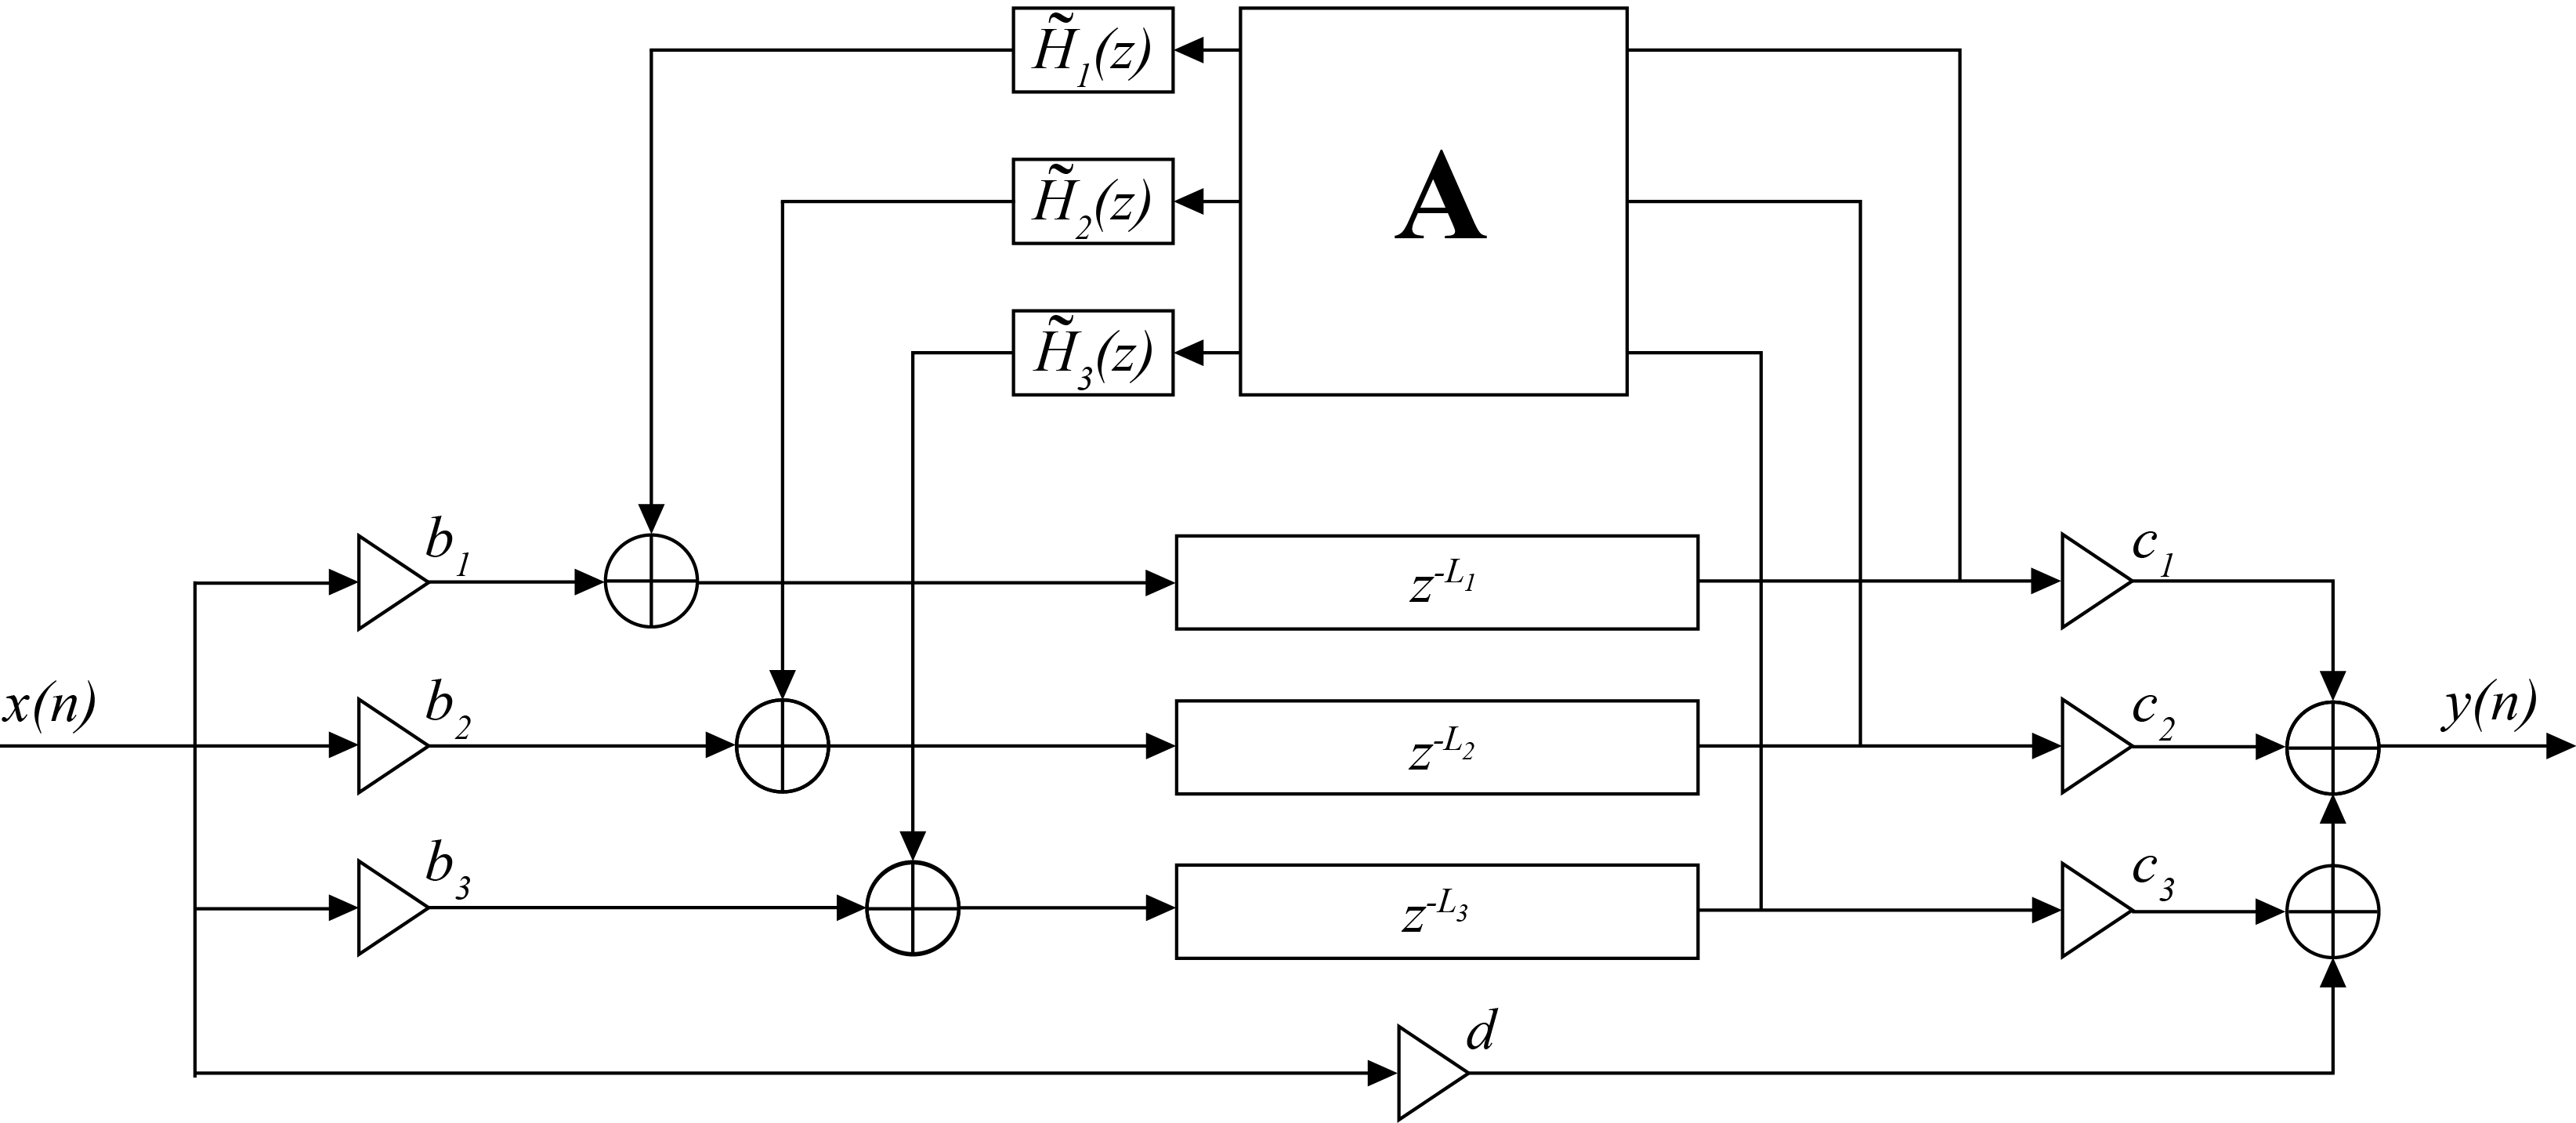
\includegraphics[scale=0.62]{Figures/diagram FDN.png}
% \caption{\textit{Flow diagram of an FDN.}}
% \label{fig:diag}
% \end{figure*}
%\begin{figure}[t!]


%\centering
%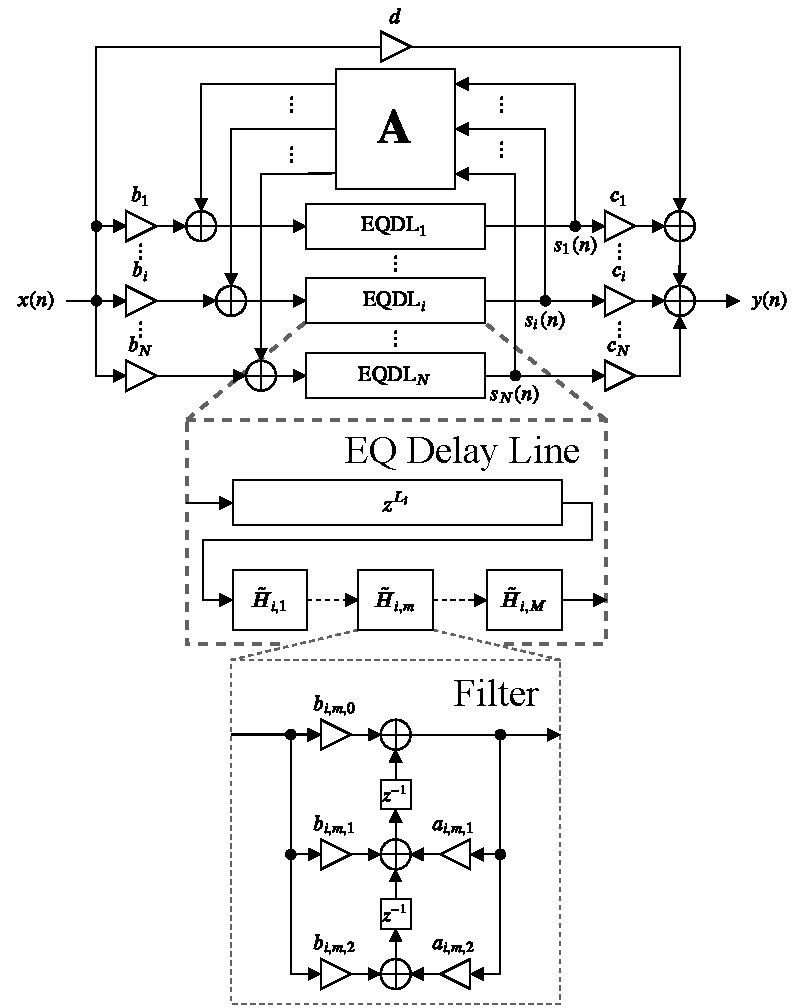
\includegraphics[scale=0.62]{Figures/FDN.pdf}
%\caption{\textit{Flow diagram of an FDN.}}
%\label{fig:diag}
%\end{figure}

The present work proposes a real-time implementation of an FDN algorithm with accurate control over reverberation time (RT) in ten octave frequency bands in the form of an audio plugin. The graphical user interface (GUI) allows a thorough insight in the attenuation filter's magnitude response, corresponding RT curve, and resulting impulse response (IR). The plugin also provides several possibilities to control the elements of FDN structure, such as feedback matrices and delay lines.% as well as the parameters of the produced sound (input gain \silvin{$\leftarrow$ might remove this}, dry/wet mix).

The paper is organised as follows: Section~\ref{sec:FDN} presents the theory behind the FDN, Section~\ref{sec:implementation} shows the GUI of the implemented plugin, describes the functionalities and user-controlled parameters of the reverberator, presents the code structure and discusses the real-time computation issues. Section~\ref{sec:resDisc} shows results regarding the echo density produced by the implementation and the CPU usage of the plugin and discusses these. Finally, Section~\ref{sec:conclusion} summarizes and concludes the work.

%\section{Background}
\section{Feedback Delay Network}\label{sec:FDN}
Figure \ref{fig:diag} presents a flow diagram of a conventional FDN, which is expressed by the relation:

\begin{subequations} \label{1}
\begin{equation}\label{1a}
y(n) =  \sum_i^N c_i s_i(n) + d x(n) 
\end{equation}
\begin{equation}\label{1b}
s_i(n + L_i) = \sum_j^N A_{i,j} \widetilde{h}_{i}(n) s_j(n) + b_i x(n),
\end{equation}
%\label{eq:fdn}
\end{subequations}
%
where $y(n)$ and $x(n)$ are the output and input signal, respectively, at time sample $n$, $s_i(n)$ is the output of the $i$th delay line, and $A_{i,j}$ is the element of an $N$th-order feedback matrix (or scattering matrix) $\textbf{A}$, through which all the delay lines are interconnected. Parameters $b_i$ and $c_i$ symbolize input and output coefficients, respectively, $d$ is the direct-path gain, and $\widetilde{h}_{i}(n)$ is the attenuation filter of the $i$th delay line.


When designing an FDN, a common practice is to first ensure that the energy of the system will not decay for any possible type of delay. Therefore, the matrix $\textbf{A}$ should be unilossless \cite{Schelcht:Habets:2017:IEEE:lossless:FDN}. To obtain a specific frequency-dependent RT, each of the delay lines must be extended by an attenuation filter, which should approximate the target gain-per-sample expressed by

\begin{equation}
	\gamma_\textrm{dB}(\omega)=\frac{-60}{f_\textrm{s} T_{60} (\omega)},
	\label{eq:gamma}
\end{equation}

\noindent where $T_{60}(\omega)$ is the target RT in seconds, $\omega = 2\pi f/f_\textrm{s}$ is the normalized frequency, $f$ is the frequency in Hz, and $f_\textrm{s}$ is the sampling rate in Hz. In order to ensure that all delay lines approximate the same RT, the gain-per-sample for each of them should be scaled by a respective delay in samples $L$, so that the following condition is met: 
\begin{equation}
	A_\textrm{dB}(\omega)=L\gamma_\textrm{dB}(\omega),
	\label{eq:attenuation}
\end{equation}

\noindent where $A_\textrm{dB}$ is the target magnitude response of the attenuation filter in dB.

In order to provide accurate approximation of the target  RT, and therefore to closely follow the $A_\textrm{dB}$, the attenuation filter used in the FDN implementation in the present study is a graphic equalizer (GEQ), which controls the energy decay of the system in ten octave bands, with center frequencies from 31.25\,Hz to 16\,kHz. The equalizer is composed of biquad filters \cite{Orfanidis:2010:introduction:SP} and designed with the method proposed by V\"alim\"aki and Liski \cite{Valimaki:Liski:2017:IEEE:accurate:equalizer} with later modifications, such as scaling by a median of gains and adding a first-order high-shelf filter as proposed in \cite{prawda:2019:improved}. The GEQ  frequency response for the $i$th delay line is expressed in dB as
\begin{equation}
    \widetilde{H}_{\textrm{dB}, i}(e^{j\omega}) = g_0+\sum_{m=1}^M \left(H_{\textrm{dB},i, m}(e^{j\omega})-\frac{g_0}{M}\right),
	\label{eq:GEQ}
\end{equation}
%
where $g_0$ is the broadband gain factor, $H_{\textrm{dB},i,m}$ are the frequency responses of the equalizing filters, and $m = 1,2,...,M$ is the frequency-band index with total number of controlled frequency bands $M$. The time domain representation of $\widetilde{H}_{\textrm{dB}, i}(e^{j\omega})$ is used as $\widetilde{h}_{i}(n)$  in Eq.~(\ref{1b}).



\begin{figure}[t!]

\centering
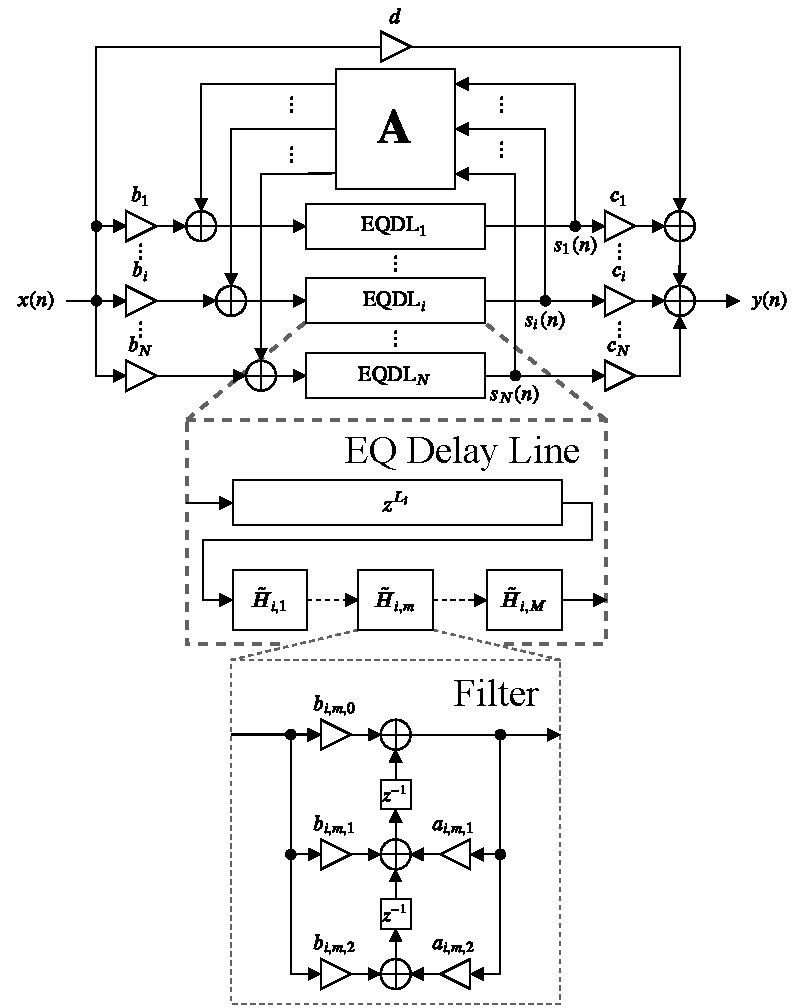
\includegraphics[width=\columnwidth]{Figures/FDN.pdf}
\caption{\textit{Flow diagram of an FDN with $N$ equalized delay lines and their $M$-octave-band biquad filters shown in detail. Here, $h_{i,m}$ is used for the time-domain representation of} $H_{\text{dB},i,m}(e^{j\omega})$\textit{ in Eq. (\ref{eq:GEQ}). See Sections \ref{sec:FDN} and \ref{sec:codeStructure} for more detailed information. }}
\label{fig:diag}
\end{figure}
%\subsection{Parameters}


\begin{figure*}[ht!]
    \centering
    \subfloat[\textit{The attenuation filter's response and the corresponding RT curve. No preset is selected and the} Smooth \textit{button is pressed. }]{\label{fig:gui}{ 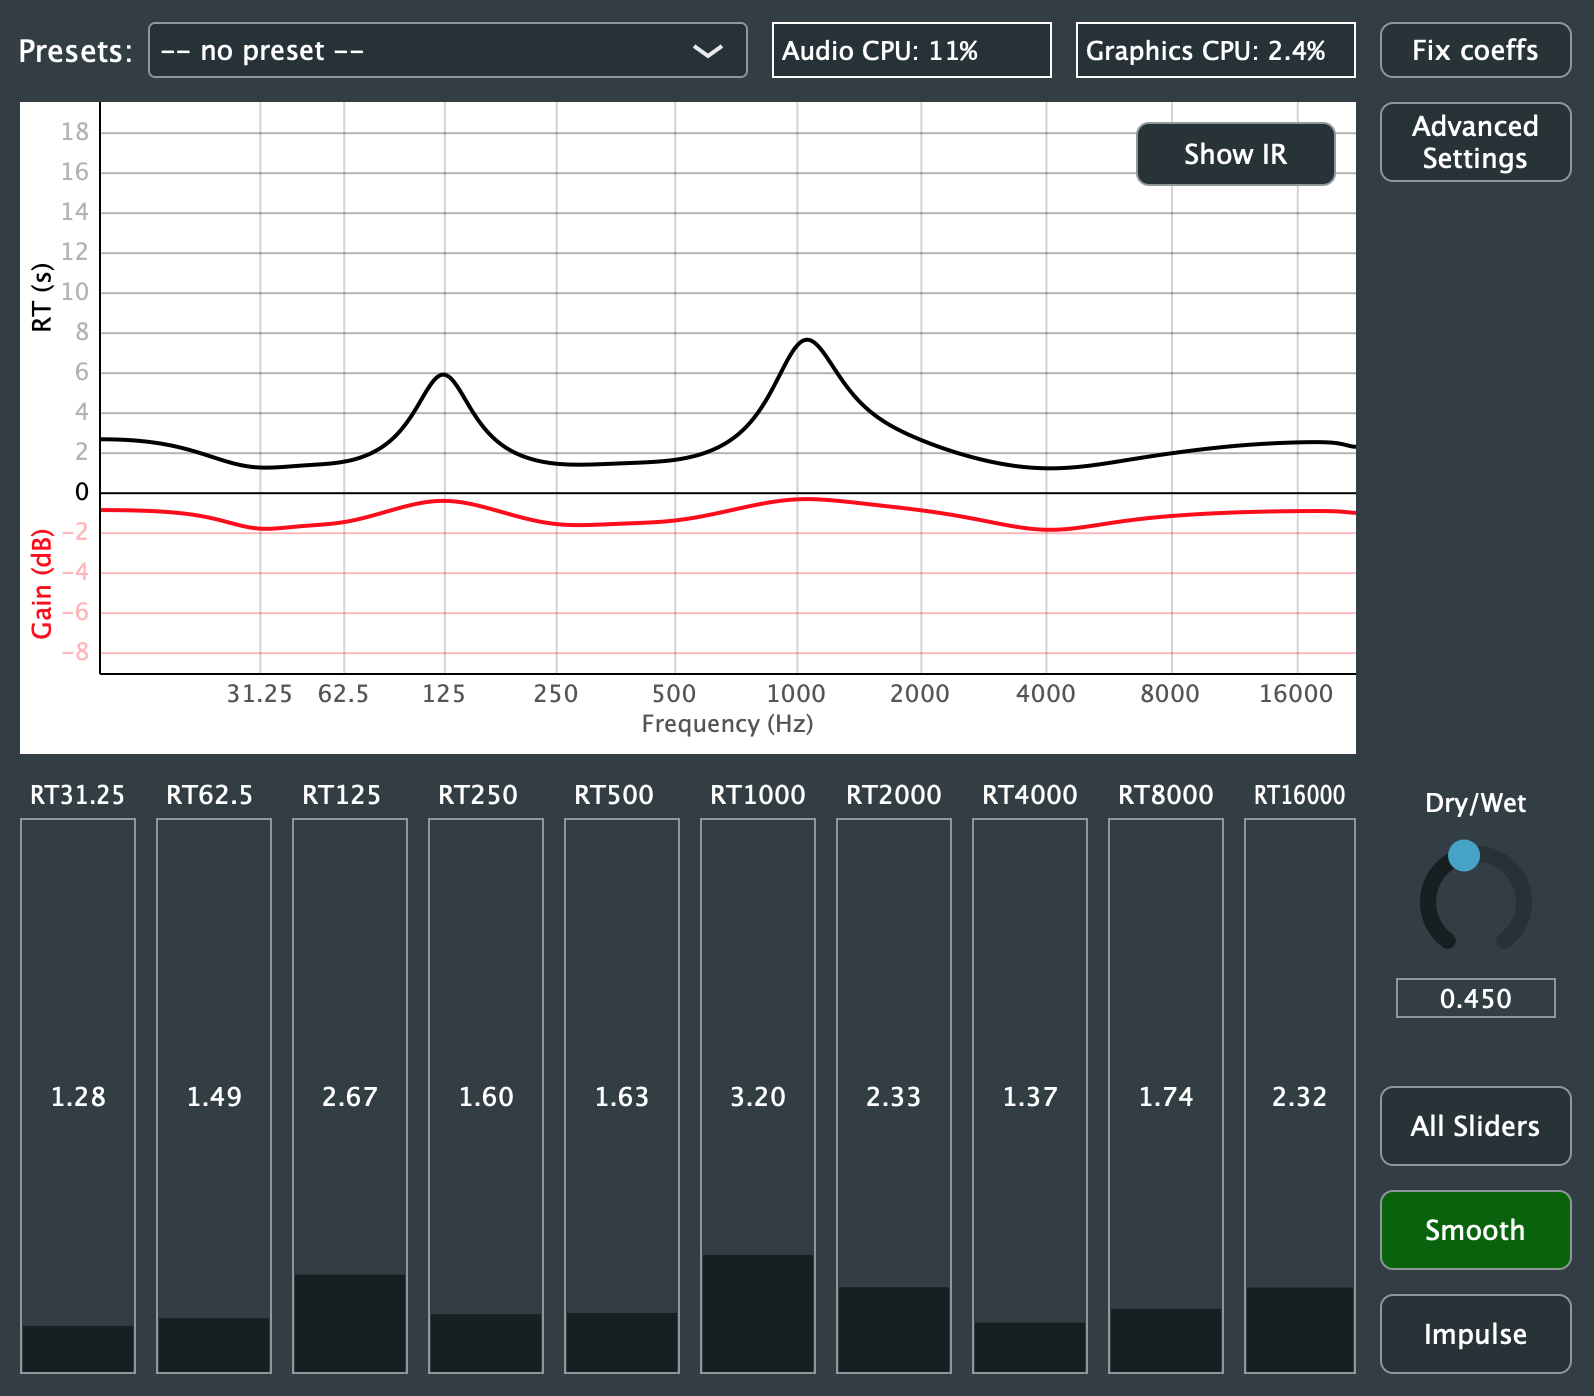
\includegraphics[width=0.48\textwidth]{Figures/GUIupdated6.png}}} \hfill
    \subfloat[\textit{The IR of the reverberator Note that the} Fix coeffs \textit{button has been pressed and the presets drop-down menu and sliders have been disabled.}]{\label{fig:gui2}{ 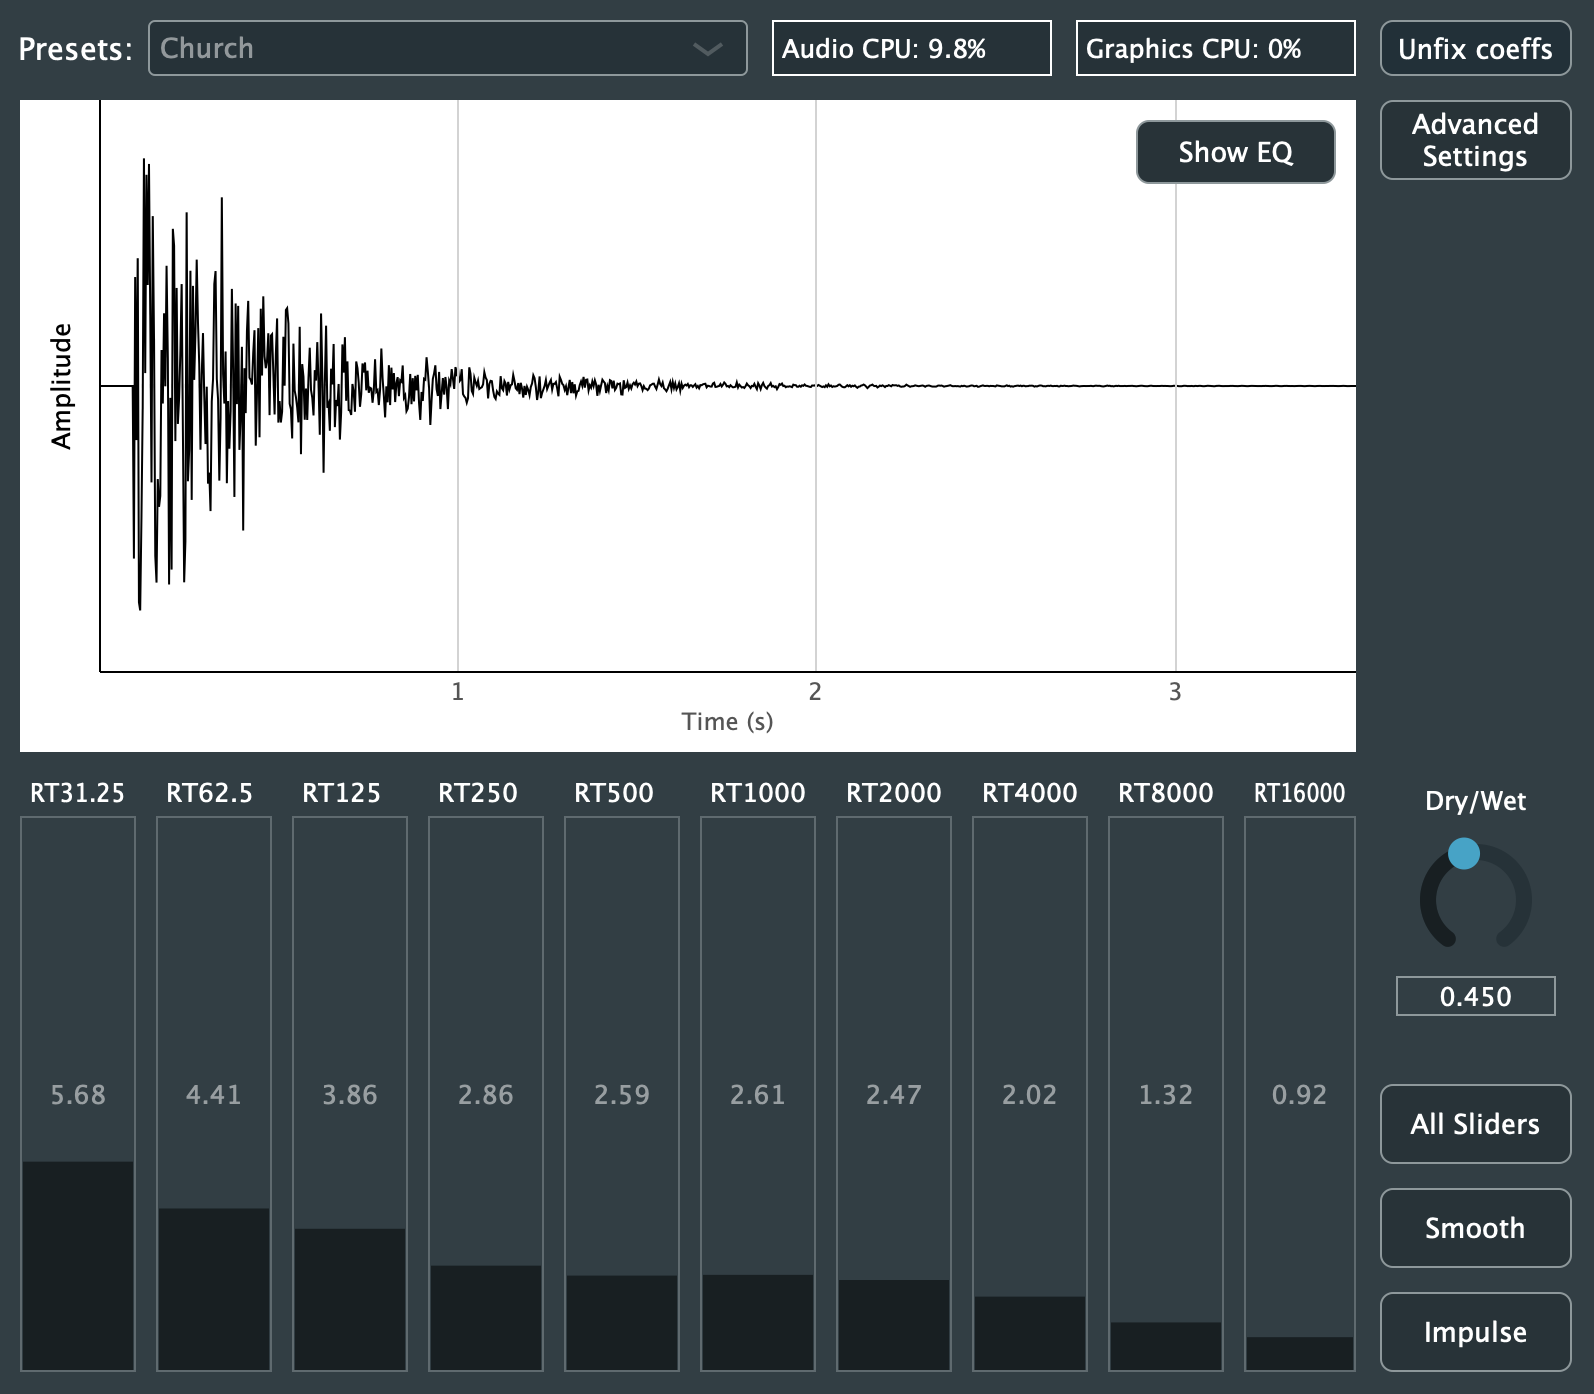
\includegraphics[width=0.48\textwidth]{Figures/GUIupdated7.png}}} \hfill
    \caption{\textit{GUI of the implemented FDN plugin.}}
    \label{fig:GUIboth}
\end{figure*}


\section{Implementation}\label{sec:implementation}

This section describes the real-time implementation of late reverberation synthesis using an FDN and a modified GEQ as the attenuation filter. The algorithm has been implemented in the form of an audio plugin  in C++ using JUCE, an open-source cross-platform application framework \cite{juce}.
% Two of the most common controls used in reverb plugins are the ratio of the (dry) input signal $d$ to the wet reverberated signal $c$ and input gain (see Eq.~\eqref{1a} and Fig.~\ref{fig:diag}). In the implementation presented in this study, those parameters are controlled by two knobs - \textit{Dry/Wet} and \textit{Input Gain}, located in the upper right part of the GUI, as shown in Fig.~\ref{fig:gui}. and~\ref{fig:gui2}. Both coefficients' values range from 0 to 1 with a 0.001 step.




% \begin{figure*}[th!]

% \centering
% 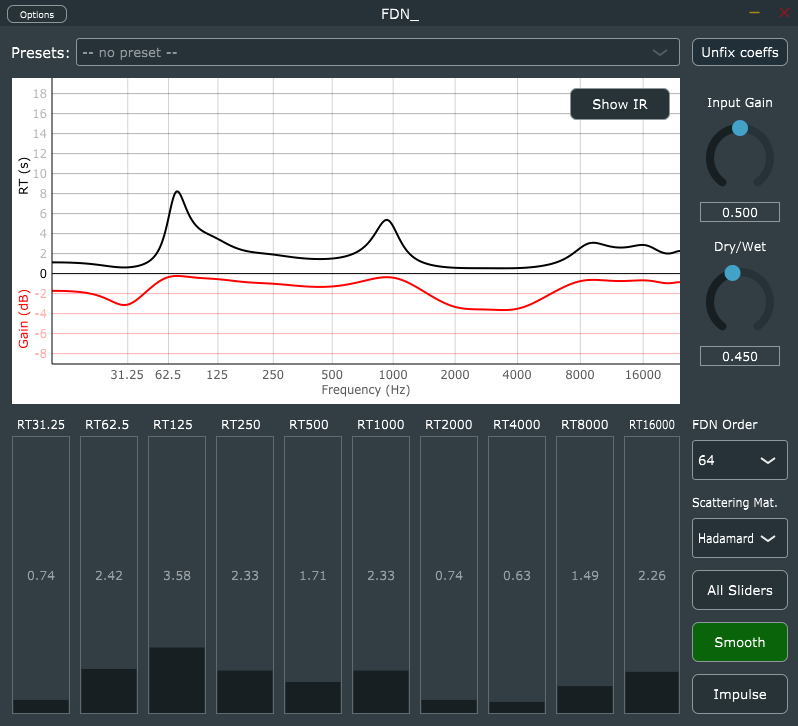
\includegraphics[scale=0.52]{Figures/gui3.png}
% \caption{\textit{ ...}}
% \label{fig:gui}
% \end{figure*}


\subsection{Control over RT Values}
In the presented implementation, the modified GEQ used as the attenuation filter allows to control the RT values in ten frequency bands. In order to utilize the whole potential of the filter, the GUI of the plugin is equipped with ten vertical sliders, each for one frequency band, as depicted in Fig.~\ref{fig:gui}. By changing the value of each of the sliders, the user is able to change the RT value for a respective frequency band from 0.03\,s to 15\,s with a 0.01\,s step. 

As too large differences between two consecutive RT values can cause instability \cite{prawda:2019:improved}, two extra modes are implemented for better control: the \textit{All Sliders} mode and the \textit{Smooth} mode. The modes are activated by pressing the respective buttons as can be seen in Fig.~\ref{fig:gui}. When either of the modes are activated, the corresponding buttons on the GUI are highlighted in green. If one mode is activated while the other already is, the other will deactivate.

The \textit{All Sliders} mode allows the user to control all the RT values to be the same by changing the slider position in one of the frequency bands. 

When the \textit{Smooth} mode is activated, changing the value of one RT will also adjust the RT in the other frequency bands. RT values of bands closer to the band that is changed will be more affected than other RT values, according to
\begin{equation}
T_{60}[m] = T_{60, \textrm{init}}[m] + \Big(T_{60}[m_\text{c}] - T_{60, \textrm{init}}[m_\text{c}]\Big) \cdot \epsilon^{|m-m_\text{c}|},
\label{eq:smooth}
\end{equation}
%
where $m_\text{c}$ is the index of currently adjusted slider, $T_{60}$ and $T_{60, \text{init}}$ are the final and initial RT values, respectively, and $\epsilon = 0.6$ is a heuristically chosen scaling factor.

In order to provide users with typical reverberation examples, five presets were created: \textit{Small Room}, \textit{Medium Room}, \textit{Large Room}, \textit{Concert Hall}, and \textit{Church}. The first three presets are based on the measurements results presented in \cite{jeub09}, whilst RT values for the last two are taken from \cite{air}. All examples are available to choose from a drop-down list in the top part of the GUI. If one of the sliders is changed, \say{-- no preset --} is displayed in the drop-down list, as shown in Fig.~\ref{fig:gui}.

The \textit{Impulse} button at the bottom right of the GUI empties the delay lines and feeds a Dirac delta into the system, so that the impulse response of the reverberator is produced as an output.

% To determine the final RT value of the $m$th frequency band, the difference between the initial and final value on the currently adjusted slider is multiplied by the scaling coefficient 0.6 raised to the power of distance between the current and $m$th slider. The result of that calculation is added to the initial number on the $m$th slider.


%\begin{figure*}[th!]

%\centering
%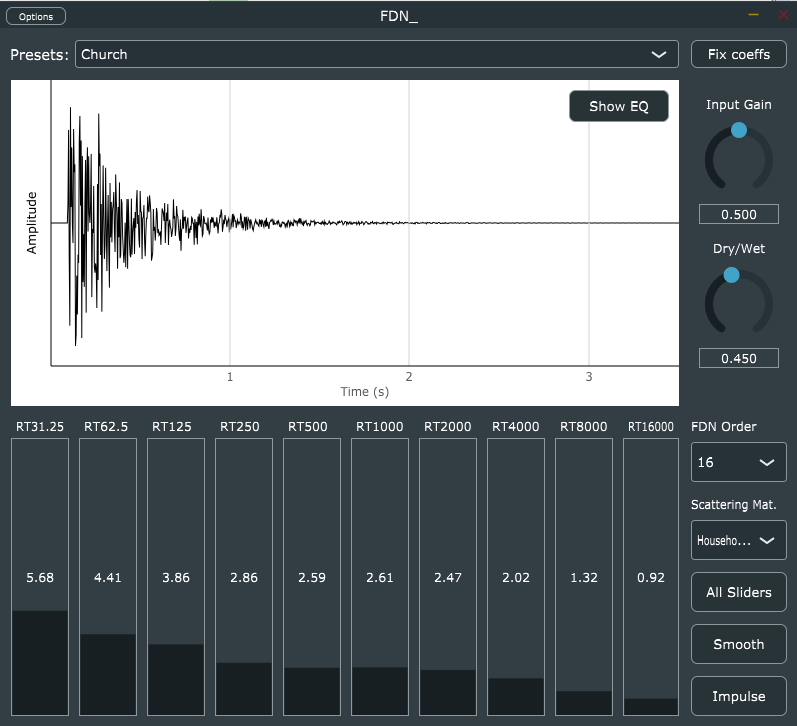
\includegraphics[scale=0.52]{Figures/GUI2.png}
%\caption{\textit{GUI of the implemented FDN plugin displaying the IR of the reverberator. }}
%\label{fig:gui2}
%\end{figure*}

\subsection{Response Plotting}
The window in the upper-half part of the plugin's GUI presented in Fig.~\ref{fig:gui} displays the RT curve (black) and the corresponding magnitude response of the attenuation filter (red), which are plotted in real time based on the values set by the sliders. This provides the user with an insight into the actual decay characteristics of the synthesised reverberation, which may differ from the user-defined RT values. This happens due to the limited ability of the attenuation filter in following the target RT curve, especially when the differences between values set for the neighbouring frequency bands are big \cite{prawda:2019:improved}. If those differences are too extreme, they may lead to the filter's magnitude response reaching 0\,dB or more, which results in the system's instability and infinite RT. This state is signaled by the background color of the window changing to light red. For the response, only one delay line is used to retain real-time plotting. Due to the fact that the attenuation filter adopts smaller values for shorter delay-line lengths, the shortest delay line is chosen as it exhibits instability sooner than the others.  


The \textit{Show IR} button located in the top right of the window allows the user to toggle between the RT curve and filter's response plots and the reverberator's IR plot, which is shown in Fig.~\ref{fig:gui2}. As opposed to the response, the longest delay line is used for calculating the IR. Even though the effect of the scattering matrix, and with that the other delay lines, are not included, it has been empirically found that using the longest delay line gives a good indication of the audible IR. The values displayed on the x-axis are determined by the average slider value, i.e., a shorter reverb time, results in a more detailed plot of the earlier seconds of the IR. Furthermore, not every sample is drawn, but 1000 data points spread over the plot range.


%\subsection{Gain control}

%Two knobs in the upper right part of the GUI control the gain of the input signal ($d$ in Equation (\ref{1a}) and Fig.~\ref{fig:diag}.) and the proportion of dry and wet signals in the output sound ($b_i$ and $c_i$ in Equations (\ref{1a}) and (\ref{1b}), and Fig.~\ref{fig:diag}.). Both coefficients' values range from 0 to 1 with 0.001 step.

\begin{figure}[t!]

\centering
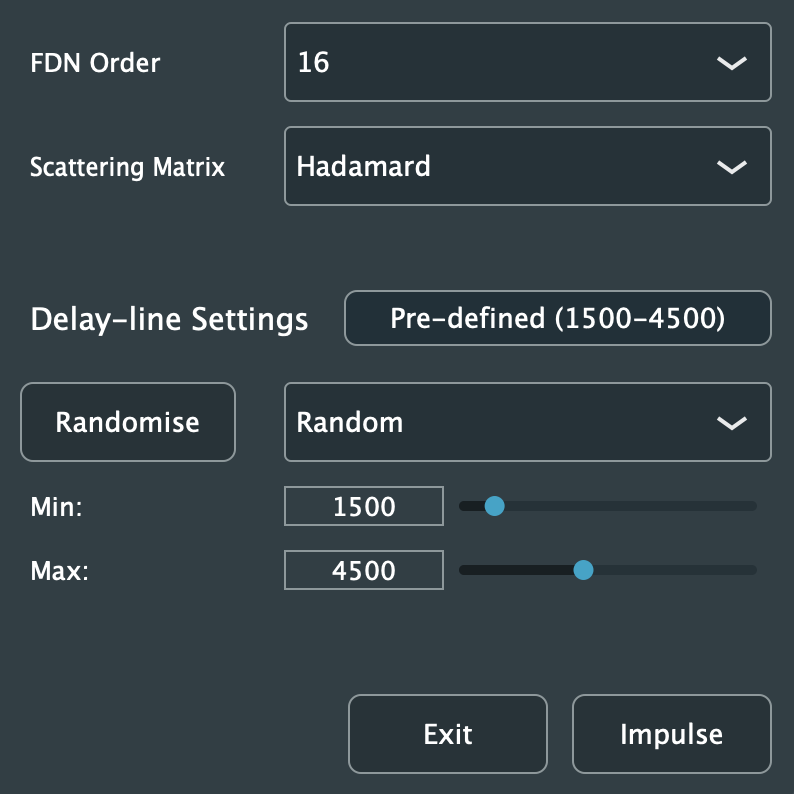
\includegraphics[width=0.8\columnwidth]{Figures/advancedSettings.png}
\caption{\textit{The advanced settings window.}}
\label{fig:advanced}
\end{figure}

\subsection{Choice of Delay Lengths and Distribution}

Although FDN-based reverbs are nowadays among the most popular algorithmic reverbs, there is no clear rule on how to choose the lengths of the delay lines \cite{Rocchesso:1997, schlecht:2016:echo}. The common practice is to choose the number of samples that are mutually prime and uniformly distributed between the maximum and minimum lengths to avoid clustering of echoes \cite{schlecht:2016:echo}. 

Through the \textit{Advanced Settings} window shown in Fig.~\ref{fig:advanced}, the distribution of delay-line lengths can be chosen among four options: \textit{Random}, \textit{Gaussian}, \textit{Primes}, and \textit{Uniform} through a drop-down menu. Whenever an option is selected, the delay-line lengths will be randomly generated based on the distribution selected. The generation can be repeated by clicking on the \textit{Randomise} button. Furthermore, the minimum (500 samples) and maximum (10,000 samples) delay-line lengths can be controlled; the minimum difference between the two has been set to 100 samples. 
Moreover, there is an option to have the lengths be pre-defined so that the plugin will have the same behavior every time it is used for all distributions. The minimum and maximum delay-line lengths have been empirically set to 1,500 and 4,500 samples respectively (\texttildelow30-100\,ms with $f_\text{s} =$  44,100\,Hz).


\subsection{Choice of Feedback Matrix}

The choice of the feedback matrix is crucial for the FDN algorithm to work correctly. The popular matrix types used in FDN implementations, which fulfill the requirement of being unilossless, are Hadamard, Householder \cite{Jot:1997:icm}, random orthogonal, and identity matrices. Where the first three are chosen to enhance specific properties of the algorithm, e.g., density of the impulse response, the identity matrix, however, reduces the FDN to a Schroeder reverberator, or a parallel set of comb filters \cite{Jot:Chaine:1991:aes, menzer2010unitary}. The plugin presented in this study allows the user to choose between those four matrices through a drop-down menu and learn about the differences in the sound obtained by changing this part of the FDN reverberator. %by clicking the button with the matrix name on the side panel in the GUI. The name depicted on the button indicates which of the matrices is currently in use.
%
Additionally, the order of the FDN, and thus the size of the feedback matrix, can be changed. The available options are 2, 4, 8, 16, 32, and 64, which can also be chosen using a drop-down menu. % In the case of Householder, when the order is changed, the delay lines are emptied to prevent any unwanted artefacts. \silvin{moved more down}

In the case of the Householder matrix type, the implementation of matrices of different sizes vary. For all orders except for 16, the matrix is constructed using following the formula:

\begin{equation}
\mathbf{A}_\textrm{N} = \mathbf{I}_\textrm{N} - \frac{2}{N} \mathbf{u}_\textrm{N}\mathbf{u}_\textrm{N}^\textrm{T},
\label{eq:house}
\end{equation}
where $\mathbf{u}_\textrm{N}^\textrm{T} = [1...1]$, and $\mathbf{I}_\textrm{N}$ is the identity matrix \cite{Jot:1997:icm}. The matrix of order 16 on the other hand, following \cite{PASPWEB2010}, is constructed using the recursive embedding of matrix of order 4:

\begin{equation}
\mathbf{A_{16}} = \frac{1}{2}
    \begin{bmatrix}
         \mathbf{A_{4}}& -\mathbf{A_{4}}& -\mathbf{A_{4}} & -\mathbf{A_{4}} \\
        -\mathbf{A_{4}} & \mathbf{A_{4}} & -\mathbf{A_{4}}& -\mathbf{A_{4}}\\
        -\mathbf{A_{4}} & -\mathbf{A_{4}} & \mathbf{A_{4}} & -\mathbf{A_{4}} \\
         -\mathbf{A_{4}} & -\mathbf{A_{4}} & -\mathbf{A_{4}} & \mathbf{A_{4}}
    \end{bmatrix}.
    \label{eq:embed}
\end{equation}
As a result, the matrix of order 16 consists of the same values, differing only in their sign.


\subsection{Code Structure}\label{sec:codeStructure}
The plugin is divided into two main components that run on different threads at different rates. Firstly, the DSP component running at 44,100\,Hz (audio rate), is structured in the same fashion as shown in Fig.~\ref{fig:diag}. A \textit{FDN} class contains the scattering matrix $\textbf{A}$ and $N$ instances of the \textit{EQDelayLine} class. This class, in turn, contains a delay line of length $L_i$ (implemented as a circular buffer) and $M$ instances of the \textit{Filter} class. This class does all the low level computation and contains the filter states and coefficients $b_{i,m}$ and $a_{i,m}$ \karolina{i think we cannot use  $b_{i,m}$ as the filter coefficients, since the same symbol is used for the coeffs in FDN in fig \ref{fig:diag} and Eq. (\ref{1b}). Maybe we should just say numerator and denominator coeffs?} of the $i$th delay line and the $m$th octave band.

Secondly, the GUI component running at 5\,Hz is responsible for the graphics and control of the FDN. Apart from the controls, this component contains the \textit{Response} class that is used for drawing the RT and gain curves and the IR shown in Figs. \ref{fig:gui} and \ref{fig:gui2}. The filter coefficients needed for drawing the curves are updated at the aforementioned rate. This calculation also provides information about the stability of the FDN and is used to trigger the light-red background denoting instability. The \textit{Response} class also contains a single instance of the \textit{EQDelayLines} class that is used for calculating the IR.

    Communication from the GUI to the DSP component happens at a 5\,Hz rate which has been found to be a great tradeoff between speed and quality of control. When changing any of the non-RT controls, the GUI triggers flags that are outside of the process buffer (512 samples) to avoid the manipulation of parameters while sample-by-sample calculations are being made. 

\begin{figure*}[t!]
    \centering
    \subfloat[\textit{Distribution of delay-line outputs for the option} Primes. ]{\label{fig:primes}{ 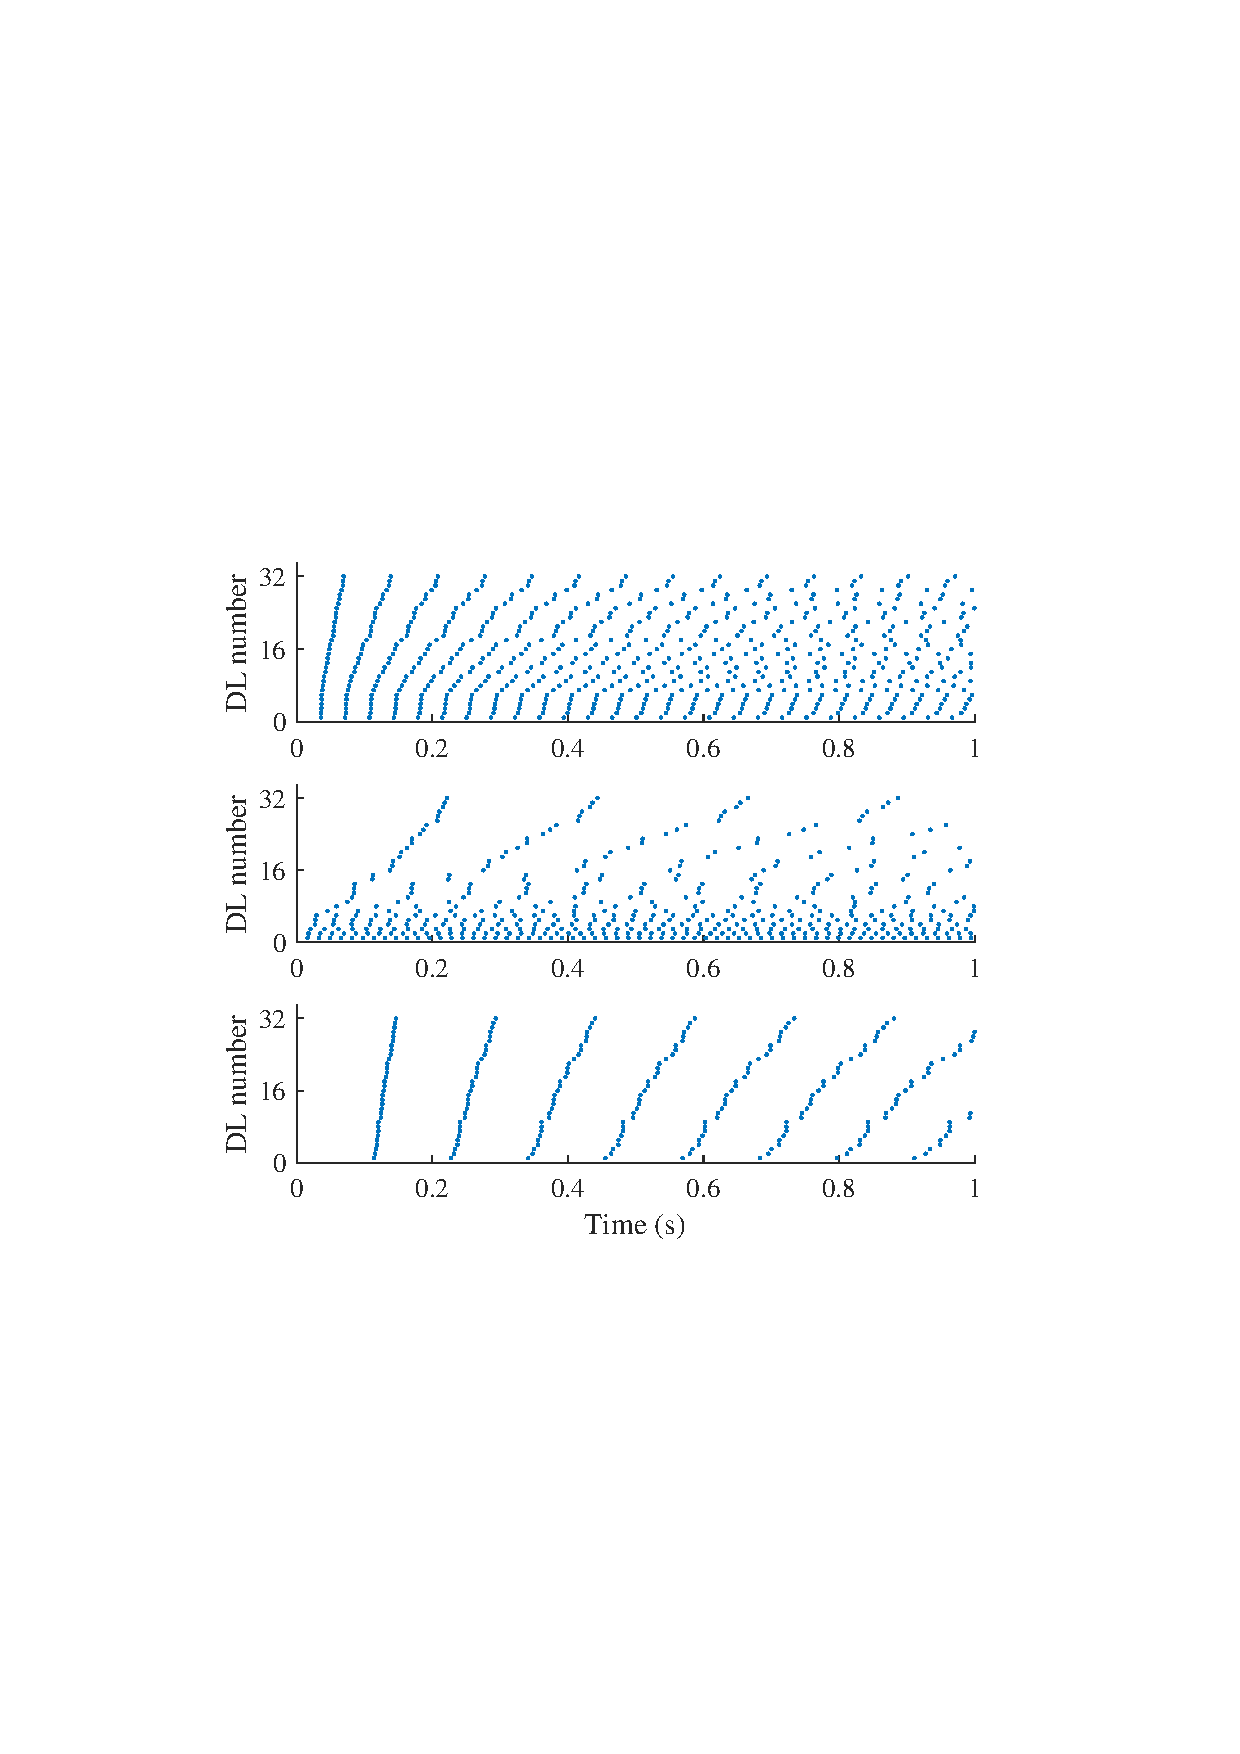
\includegraphics[trim=4.2cm 8.8cm 4.2cm 9cm, width=0.42\textwidth]{Figures/primes.pdf}}} \hfill
    \subfloat[\textit{Distribution of delay-line outputs for the option} Uniform. ]{\label{fig:uniform}{ 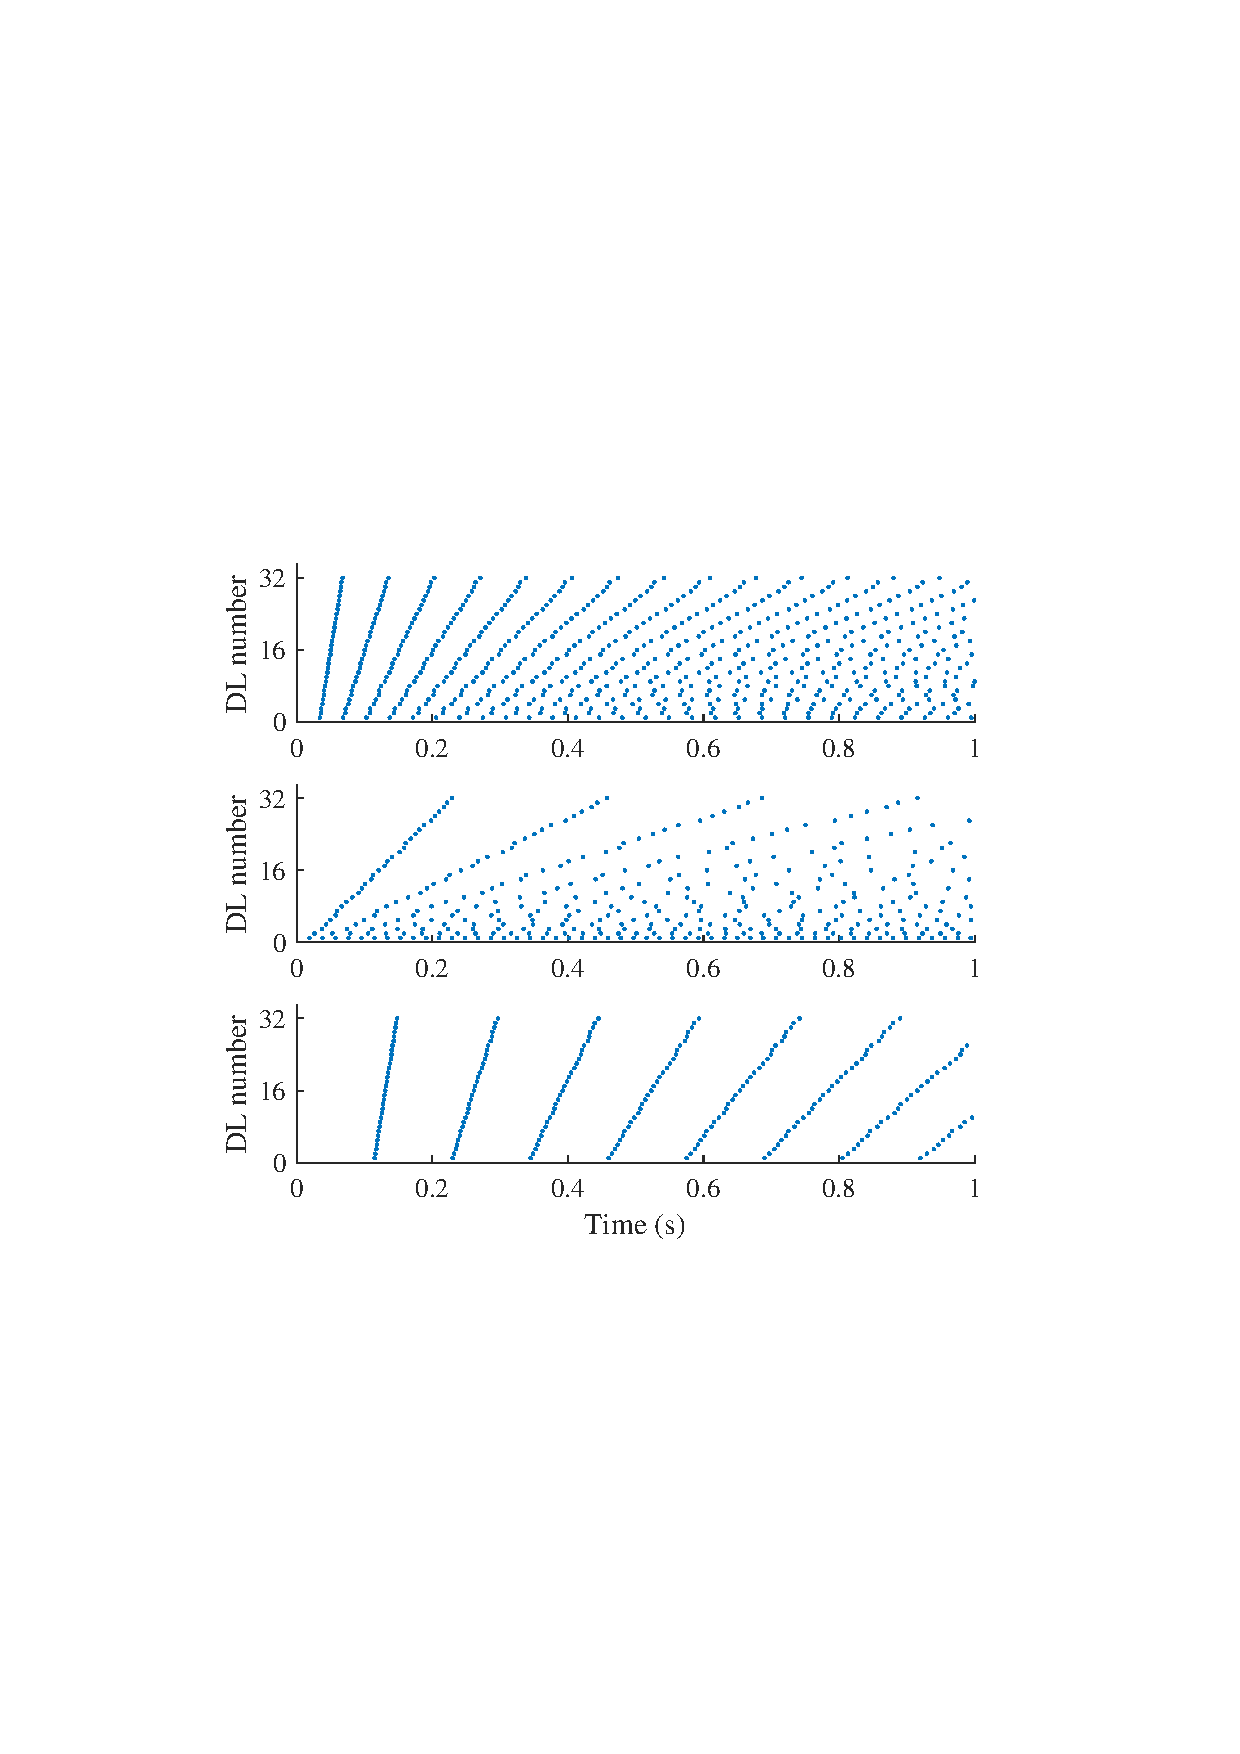
\includegraphics[trim=4.2cm 8.8cm 4.2cm 9cm, width=0.42\textwidth]{Figures/uniform.pdf}}} \hfill
    \subfloat[\textit{Distribution of delay-line outputs for the option} Random. ]{\label{fig:random}{ 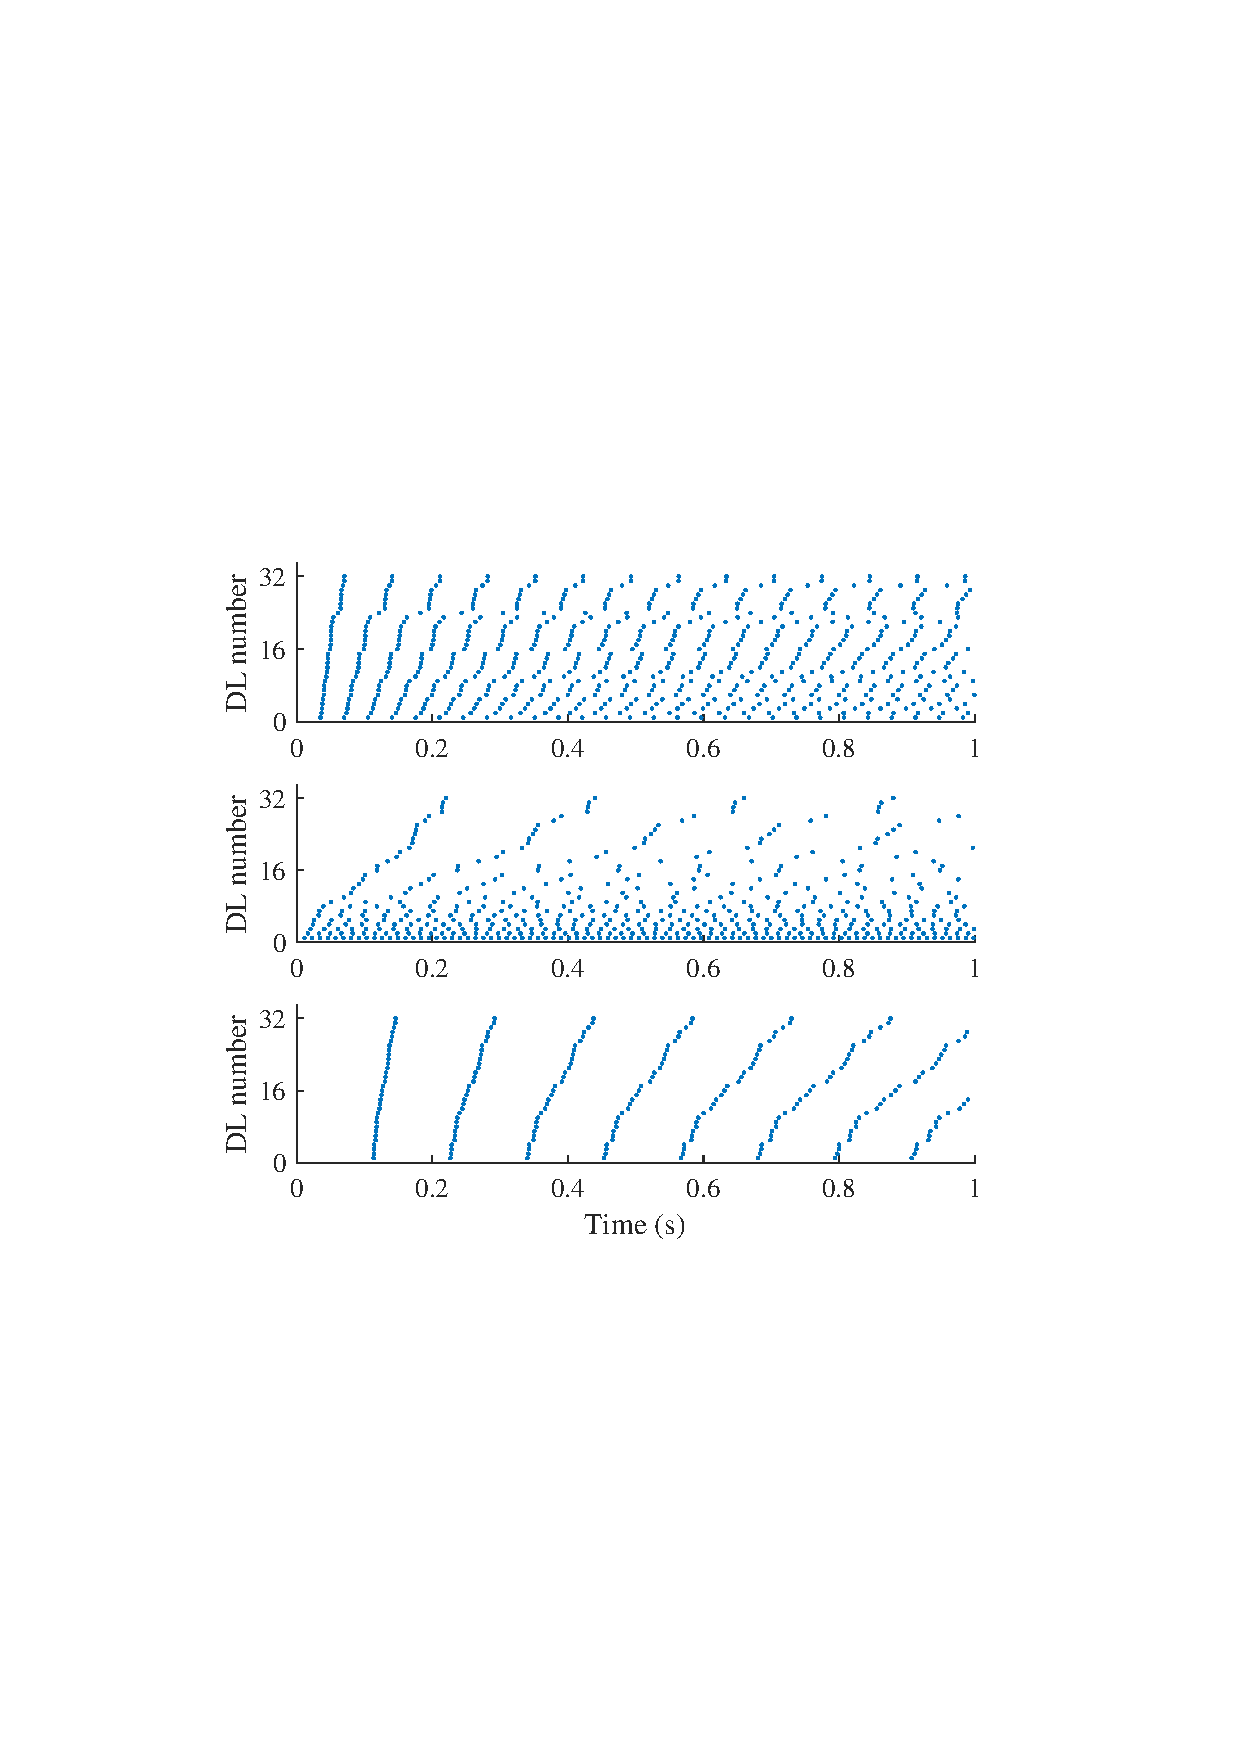
\includegraphics[trim=4.2cm 8.8cm 4.2cm 9cm, width=0.42\textwidth]{Figures/random.pdf}}} \hfill
    \subfloat[\textit{Distribution of delay-line outputs for the option} Gaussian. ]{\label{fig:gauss}{ 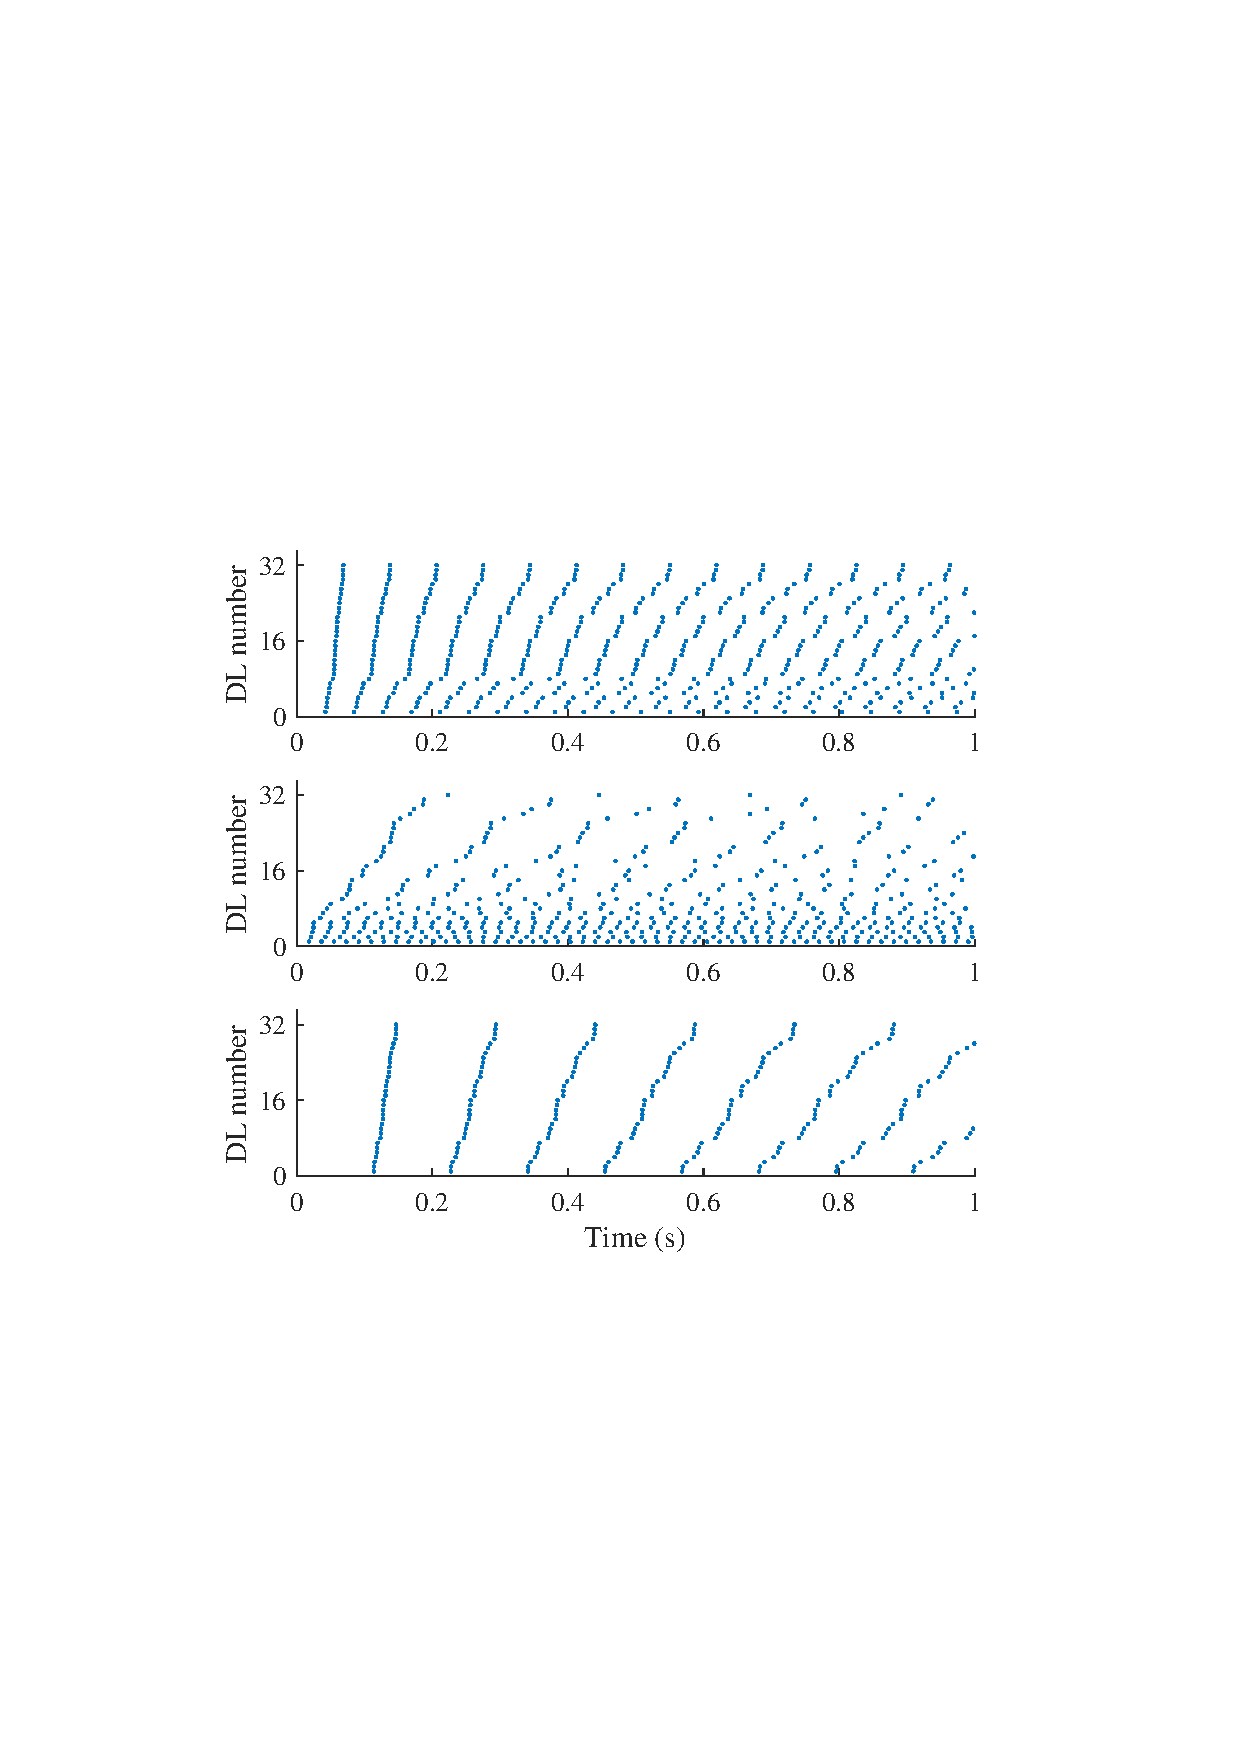
\includegraphics[trim=4.2cm 8.8cm 4.2cm 9cm, width=0.42\textwidth]{Figures/gaussian.pdf}}}
    \caption{\textit{The distribution of the outputs of 32 delay lines depending on the chosen option and length range (assuming no scattering is present). The dots mark the time unit in which the given delay-line outputs a sample. (Top panes) Pre-defined lengths (1,500--4,500 samples). (Middle panes) Lengths randomised over the whole range (500--10,000 samples). (Bottom panes) Lengths randomised over a narrow range (5,000--6,500 samples). }}
    \label{fig:dLens}
\end{figure*}

\subsection{Real-time Considerations}
The components of the plugin requiring most computations are the (re-)calculation of the filter coefficients and the plotting of the responses. Even though the filter coefficients only need to be recalculated when slider values are changed, it is good practice for a plugin to have the same CPU usage when its values are changed as when its values are static to prevent unexpected spikes in the CPU usage. Instead, a \textit{Fix coeffs} (coefficients) button has been implemented that, when clicked, will deactivate the presets drop-down menu and the sliders (as shown in Fig.~\ref{fig:gui2}). Furthermore, the plugin will stop recalculating the plots and filter coefficients, greatly decreasing CPU usage (see Sec.~\ref{sec:resDisc} \silvin{$\leftarrow$ Would this be referring to the table of cpu usage that I still need to add?} \karolina{I thought that you put this here? I think I haven't written anything in this section} \silvin{Haha probably I wrote it a while ago.. Doing it now!}). The CPU usages of each individual thread are shown at the top of the plugin.

When any change is made to the FDN, be it the order, delay-line distribution or length, the delay lines and filter states are set to zero to prevent any unwanted artefacts. Only the RT control works in real time without emptying the delay lines and filter states.

\section{Results and Discussion}\label{sec:resDisc}

This section will present results regarding the echo density produced by the implementation and plugin's CPU usage and discuss these.

\subsection{Echo Density}
To achieve smooth reverberation, a sufficient echo density, i.e., the number of echoes per time unit produced by the algorithm and their distribution \cite{schlecht:2016:echo}, should be obtained. Echo density is affected by a few factors, such as the lengths and the distribution of the delay lines, the type of the feedback matrix and its size, all of which is discussed below.

\subsubsection{Behavior with Different Choices of Delay Lines}
The practice of choosing mutually prime delay-line lengths is aimed at avoiding more than one sample appearing at the system's output at the same time, and clustering the echoes, since both of these phenomena lower the echo density. Using this delay-line distribution does not, however, always ensure smooth reverberation. Their distribution and the range over which they are chosen are also the factors affecting the quality of the synthesised sound. The distribution of delay-line outputs over time, assuming no scattering is present, is shown in Fig.~\ref{fig:dLens} for all the options available in the plugin. The delay-line lengths were sorted in an ascending order.

The top panes of the Figures~\ref{fig:primes}.-\ref{fig:gauss}. show the outputs of the pre-defined delay lines, which depicts the typical behavior of the FDN algorithm. The outputs become more diffused over time, making the reverb smoother. In the uniform distribution, where the consecutive delay-line lengths differ by a constant number of samples, the phenomena of output samples overlapping is inevitable. 

The distribution of outputs presented in the middle panes show that when the delay-lengths range is very wide, the output is diffused from the beginning. As such decay is rarely met in reality, it is useful when recreating only specific spaces \cite{Oksanen13}. Additionally, very short delay lines create clusters of echoes and huge portion of the output samples overlap. They do not contribute to the increase of echo density, but nevertheless add to the computation. Such clusters are well visible in Fig.~\ref{fig:primes} and~\ref{fig:random}. Moreover, the attenuation applied to the short delay lines is usually small, and therefore closer to 0 dB, which makes them more prone to causing the system's instability.

On the other hand, very long delay lines (10,000 samples translates to ca. 0.23\,s) may not introduce meaningful contribution to the synthesised reverb in case of low RT values. However, such long delay lines still add the computation, since the size of the feedback matrix needs to be equal to the number of delay lines.

Using a very narrow range over which the delay-line lengths are distributed results in clusters of samples arriving at the output within very short time, as depicted in the bottom panes of Fig.~\ref{fig:dLens}. Between the consecutive clusters, however, long periods of zeros occur. The synthesised reverberation tail diffuses very slowly, which results in low-quality sound with clearly audible segmentation. When such narrow range, the effect behavior resembles more that of a single delay line than a reverb. 




\subsubsection{Effect of Feedback Matrix on Echo Density}\label{subsubsec:feedbackMatrix}

The normalized echo densities for all types of matrices available in the plugin were calculated, following the method presented in \cite{abel:2006, huang:2007, huang:2008}, for orders 2--64 and the delay lines selected randomly %from a uniform distribution 
from the range between 1,500 and 4,500 samples (the same set of delay lines was used for all calculations). The results are depicted in Fig.~\ref{fig:echo} which generally show that the echo density increases faster with a higher FDN order than with a lower one. 

When matrices of size 2 and 4 are used, the number of echoes in the output of the reverberator increases slowly and may never reach saturation, i.e. a moment, when there is an echo at every successive time unit \cite{schlecht:2016:echo}. Therefore, those low orders do not produce smooth sound. In the case of an FDN of order 8, the echo density build-up is slow, which results in audible artifacts in synthesized reverbs for as long as one second. Thus, a matrix of size 16 is the smallest that increases the number of echoes quickly enough so that the resulting sound is perceived as smooth for all matrix-types (except for the identity matrix). For the Hadamard and random matrices, further rise in the size accelerates the echo density build-up, as depicted in Fig.~\ref{fig:echoHad} and~\ref{fig:echoRand}.

Interestingly, the Householder matrix excels with the order of 16 using the recursive embedding shown in Eq.~\eqref{eq:embed}. This can be explained by the fact that for all other orders the implementation is according to Eq.~\eqref{eq:house} which produces matrices in which the difference between the diagonal and the rest of the elements grows proportional to the order. Effectively, this makes the FDN approach a bank of decoupled comb filters. This results in high variability of echo density for orders 32 and 64, as depicted in Fig.~\ref{fig:echoHouse} and leads to audible artifacts in the reverberation. For the matrix of order 16, however, the echo density increases faster and is more stable once it reaches saturation.

Because of the fact that the identity matrices produce a very low echo density that does not increase with time, as shown is Fig.~\ref{fig:echoIde}, they are not well fitted for the FDN. Reverberation synthesised using such matrices is always low-quality.  Due to the fact that the Householder matrix of order 2 is also an identity matrix, it also should be avoided when the target is to obtain smooth, high-quality sound. 
\begin{figure*}[ht!]
    \centering
    \subfloat[\textit{Identity matrix.}]{\label{fig:echoIde}{ 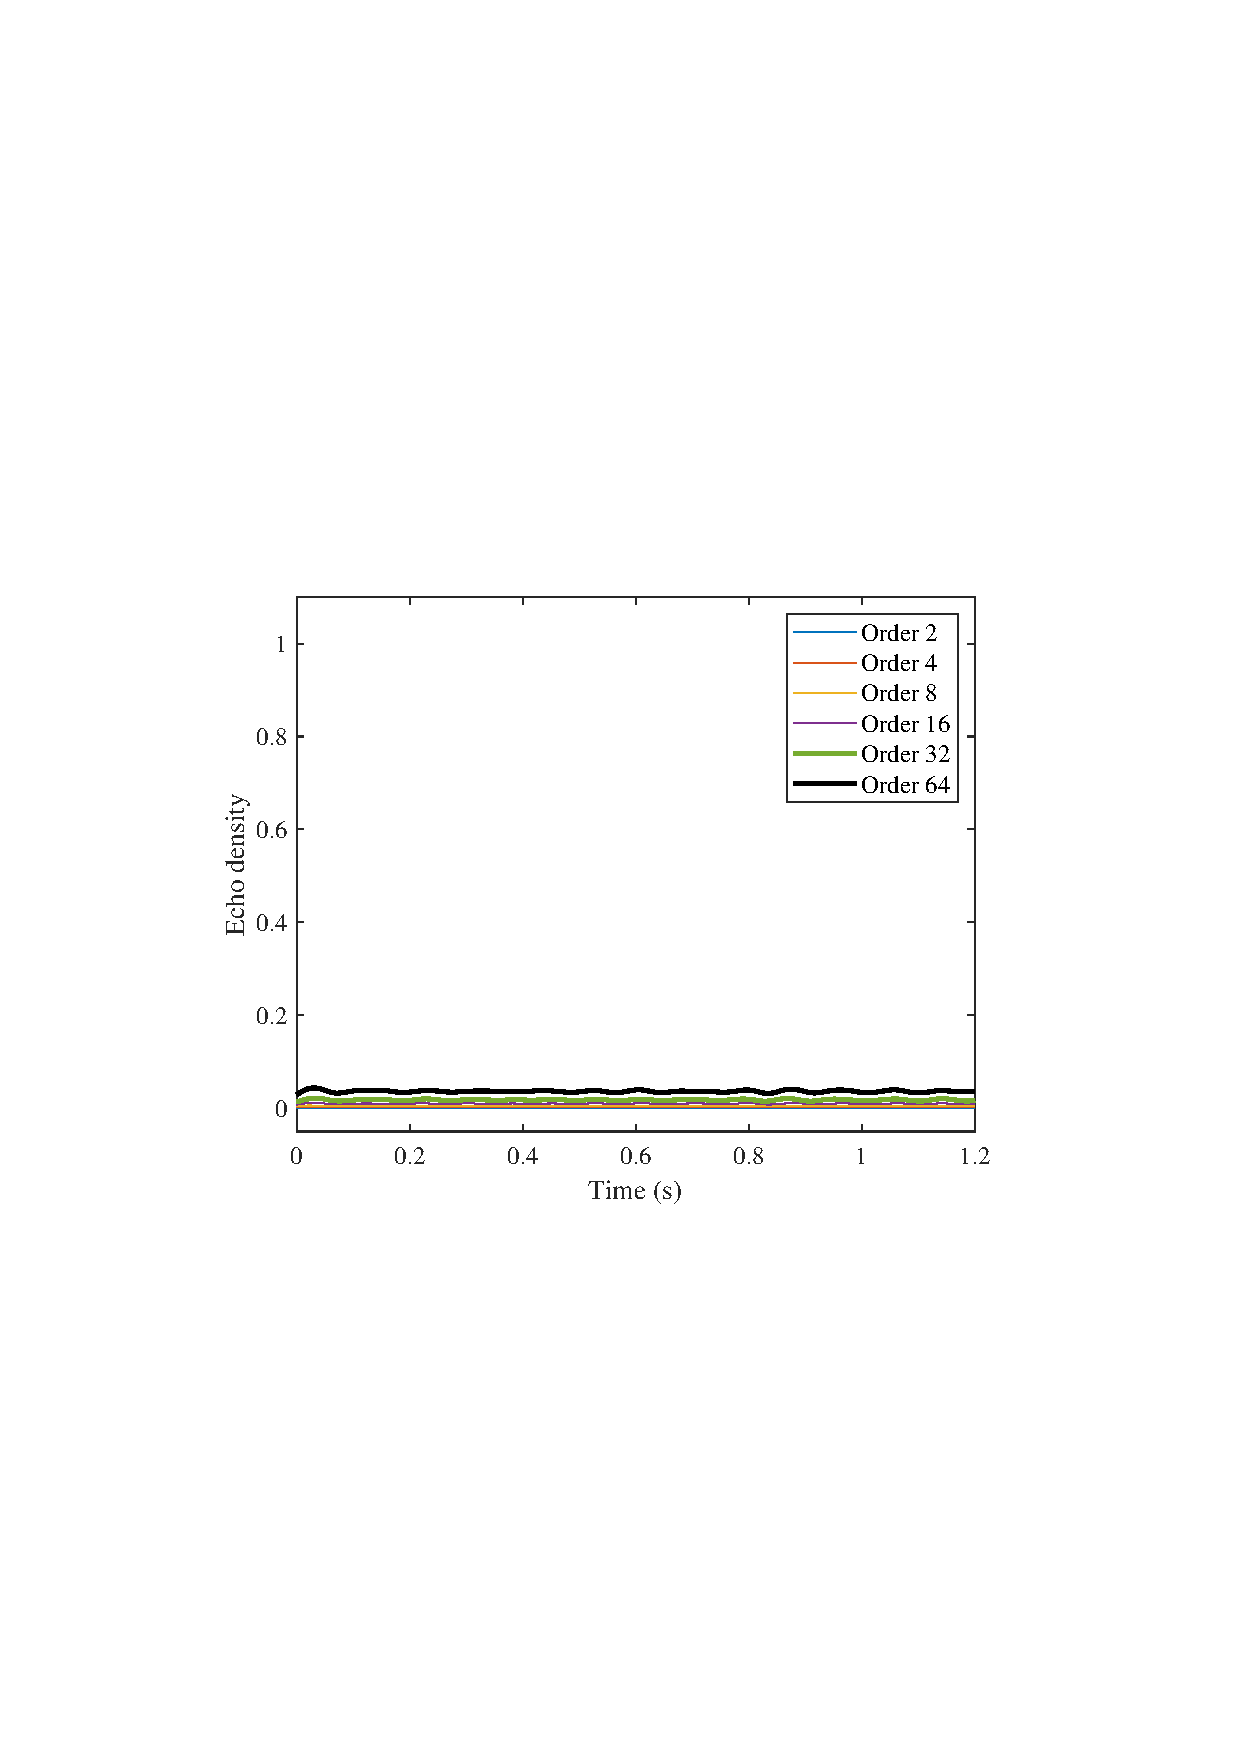
\includegraphics[trim=4cm 9.2cm 4.2cm 10cm, width=0.44\textwidth]{Figures/echoIde.pdf}}}\hfill
    \subfloat[\textit{Householder matrix.}]{\label{fig:echoHouse}{ 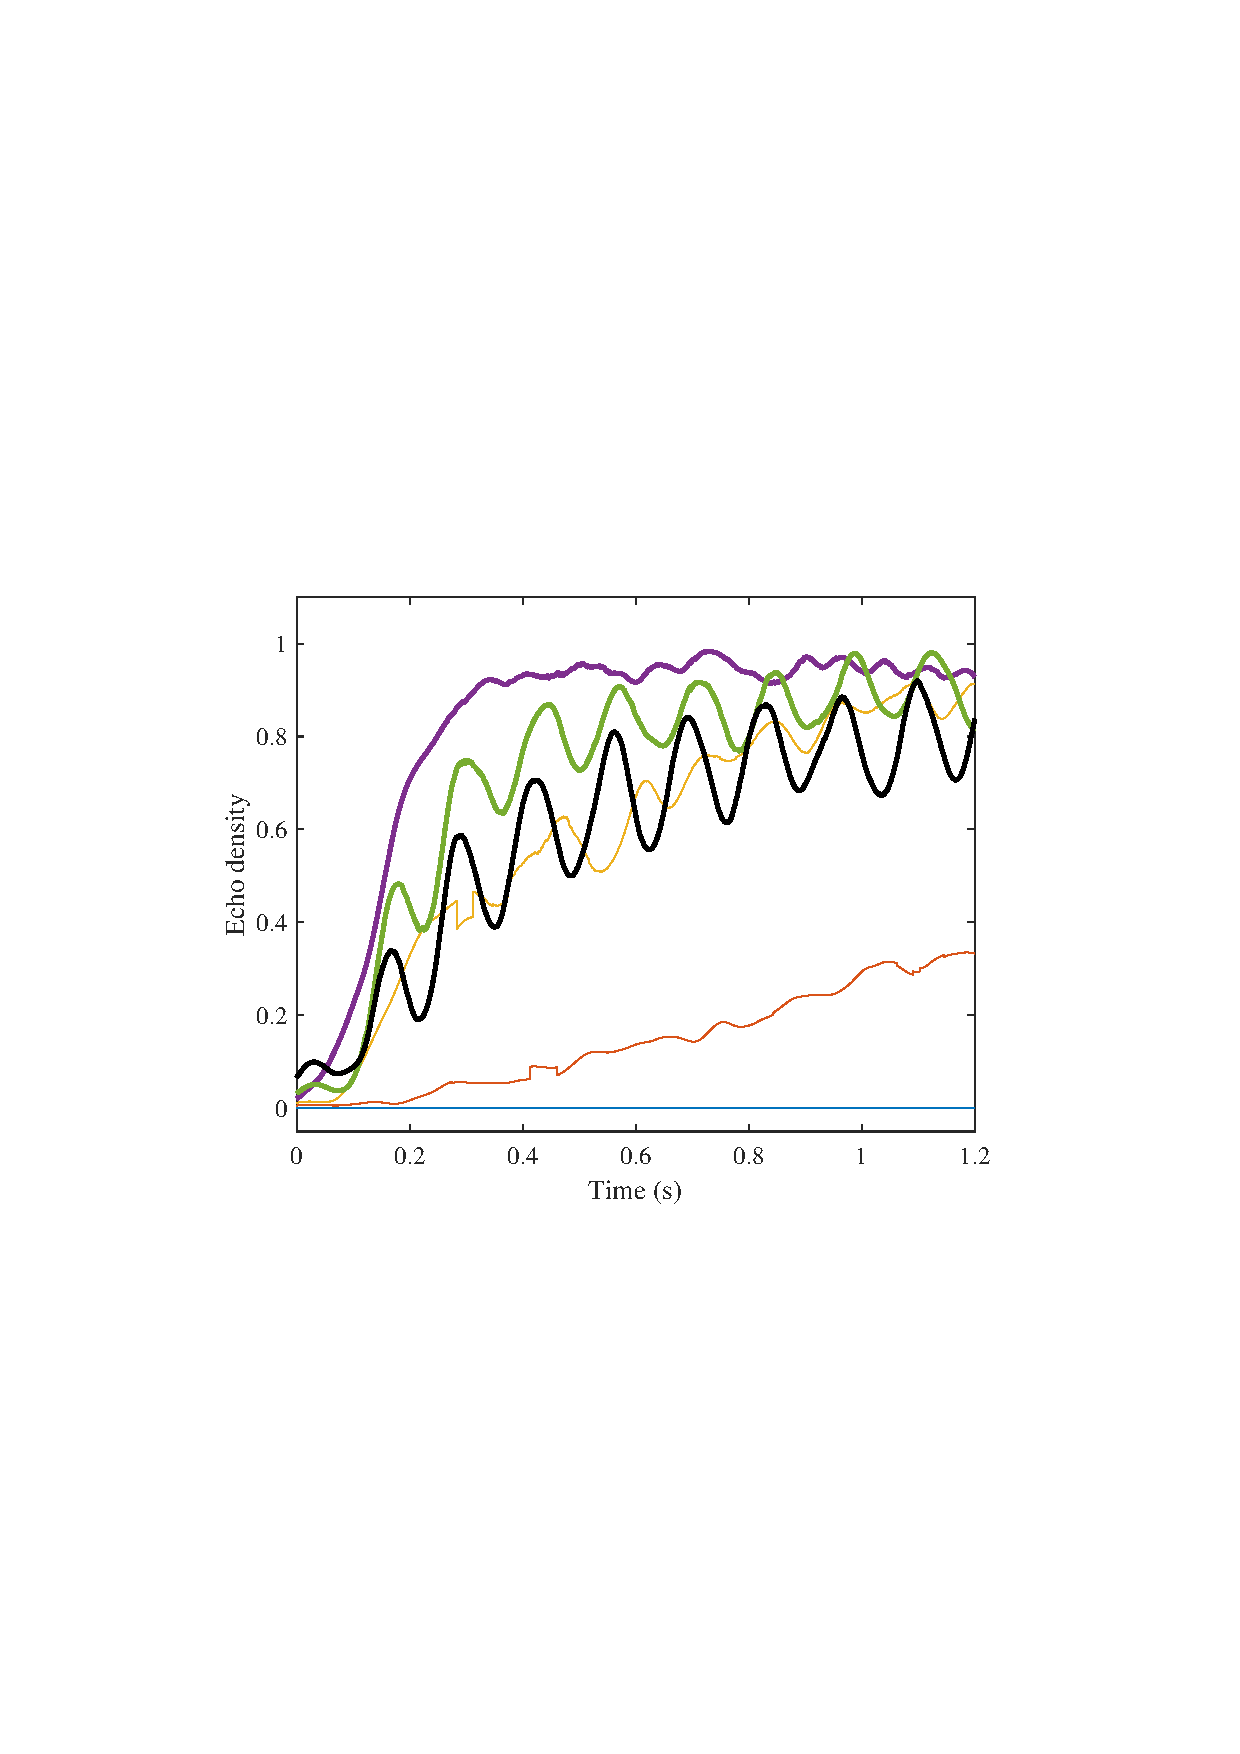
\includegraphics[trim=4.cm 9.2cm 4.2cm 10cm, width=0.44\textwidth]{Figures/echoHouse.pdf}}} \hfill
    \subfloat[\textit{Hadamard matrix.}]{\label{fig:echoHad}{ 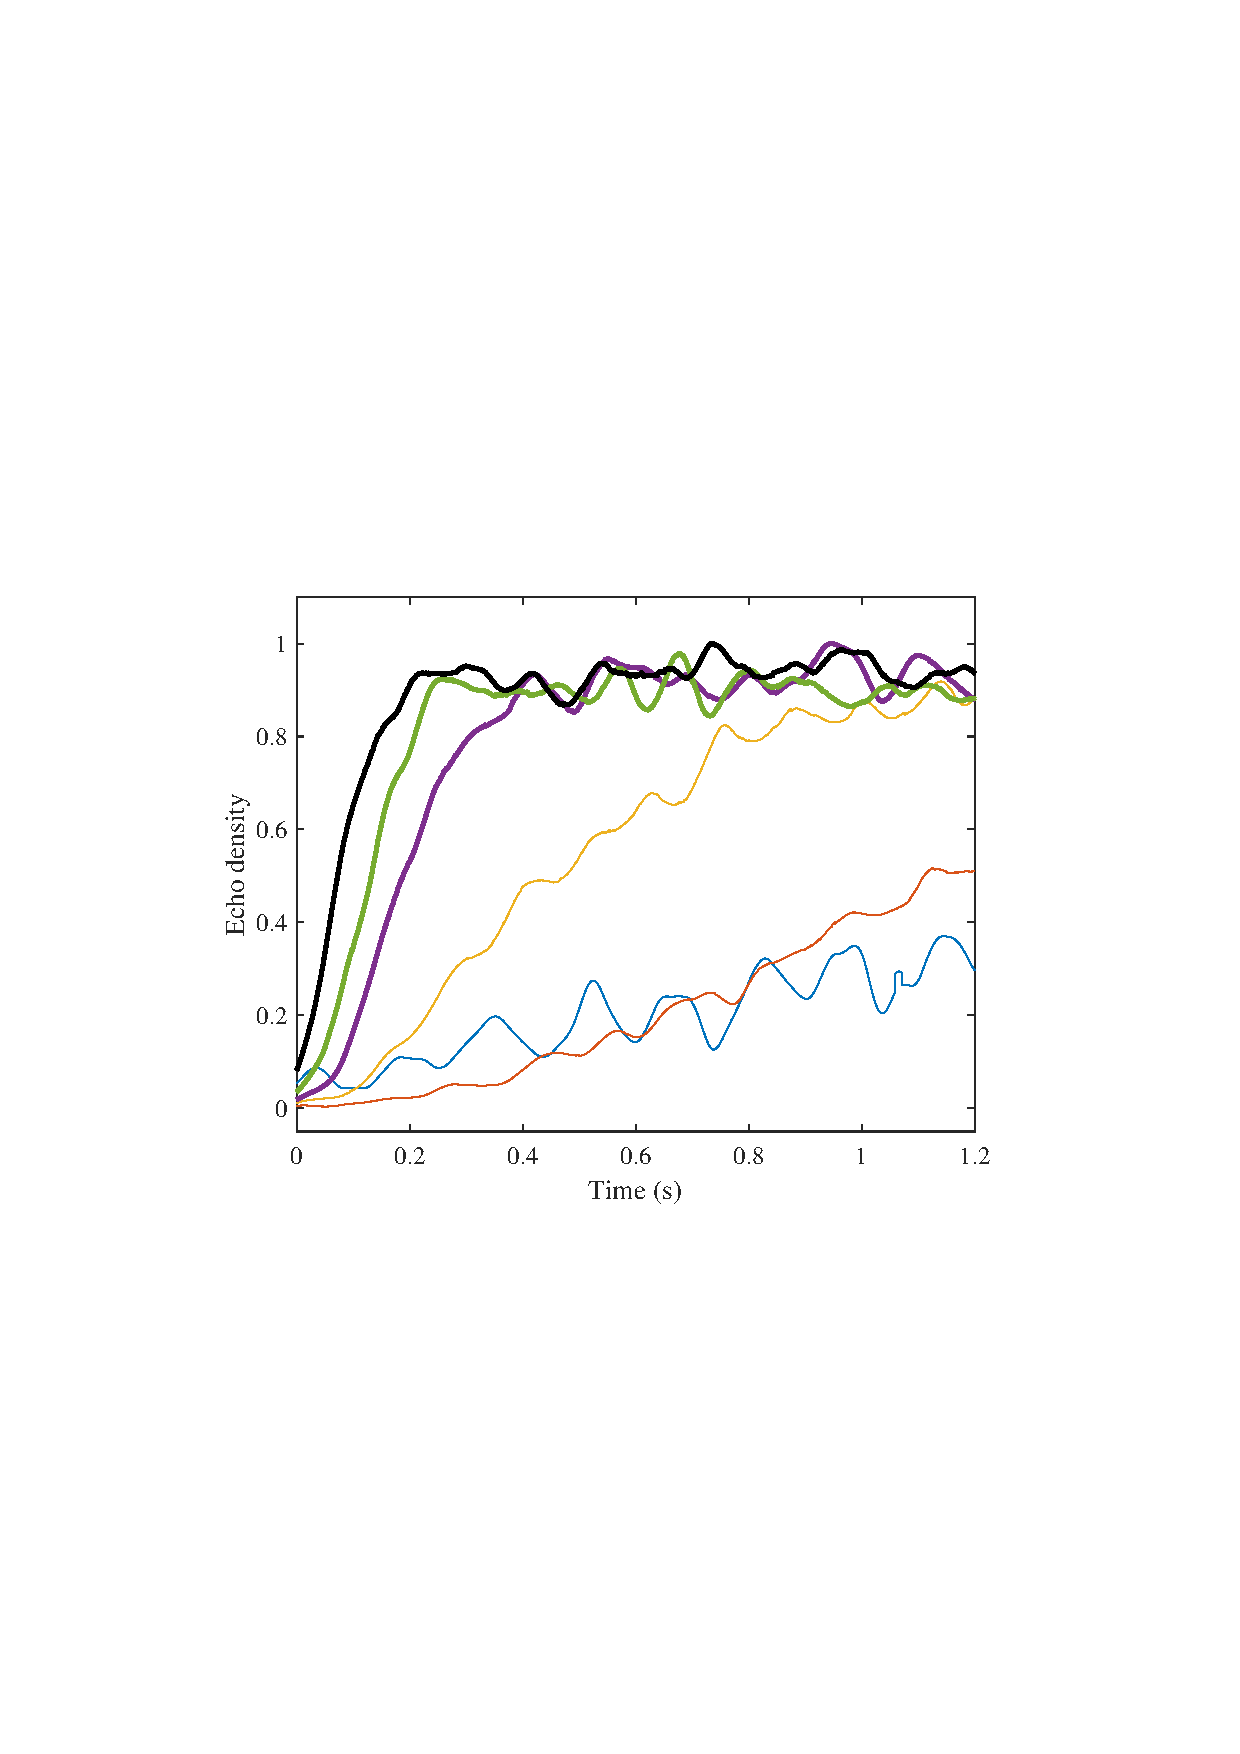
\includegraphics[trim=3.8cm 9.2cm 4.5cm 10cm, width=0.44\textwidth]{Figures/echoHad.pdf}}} \hfill
    \subfloat[\textit{Random orthogonal matrix.}]{\label{fig:echoRand}{ 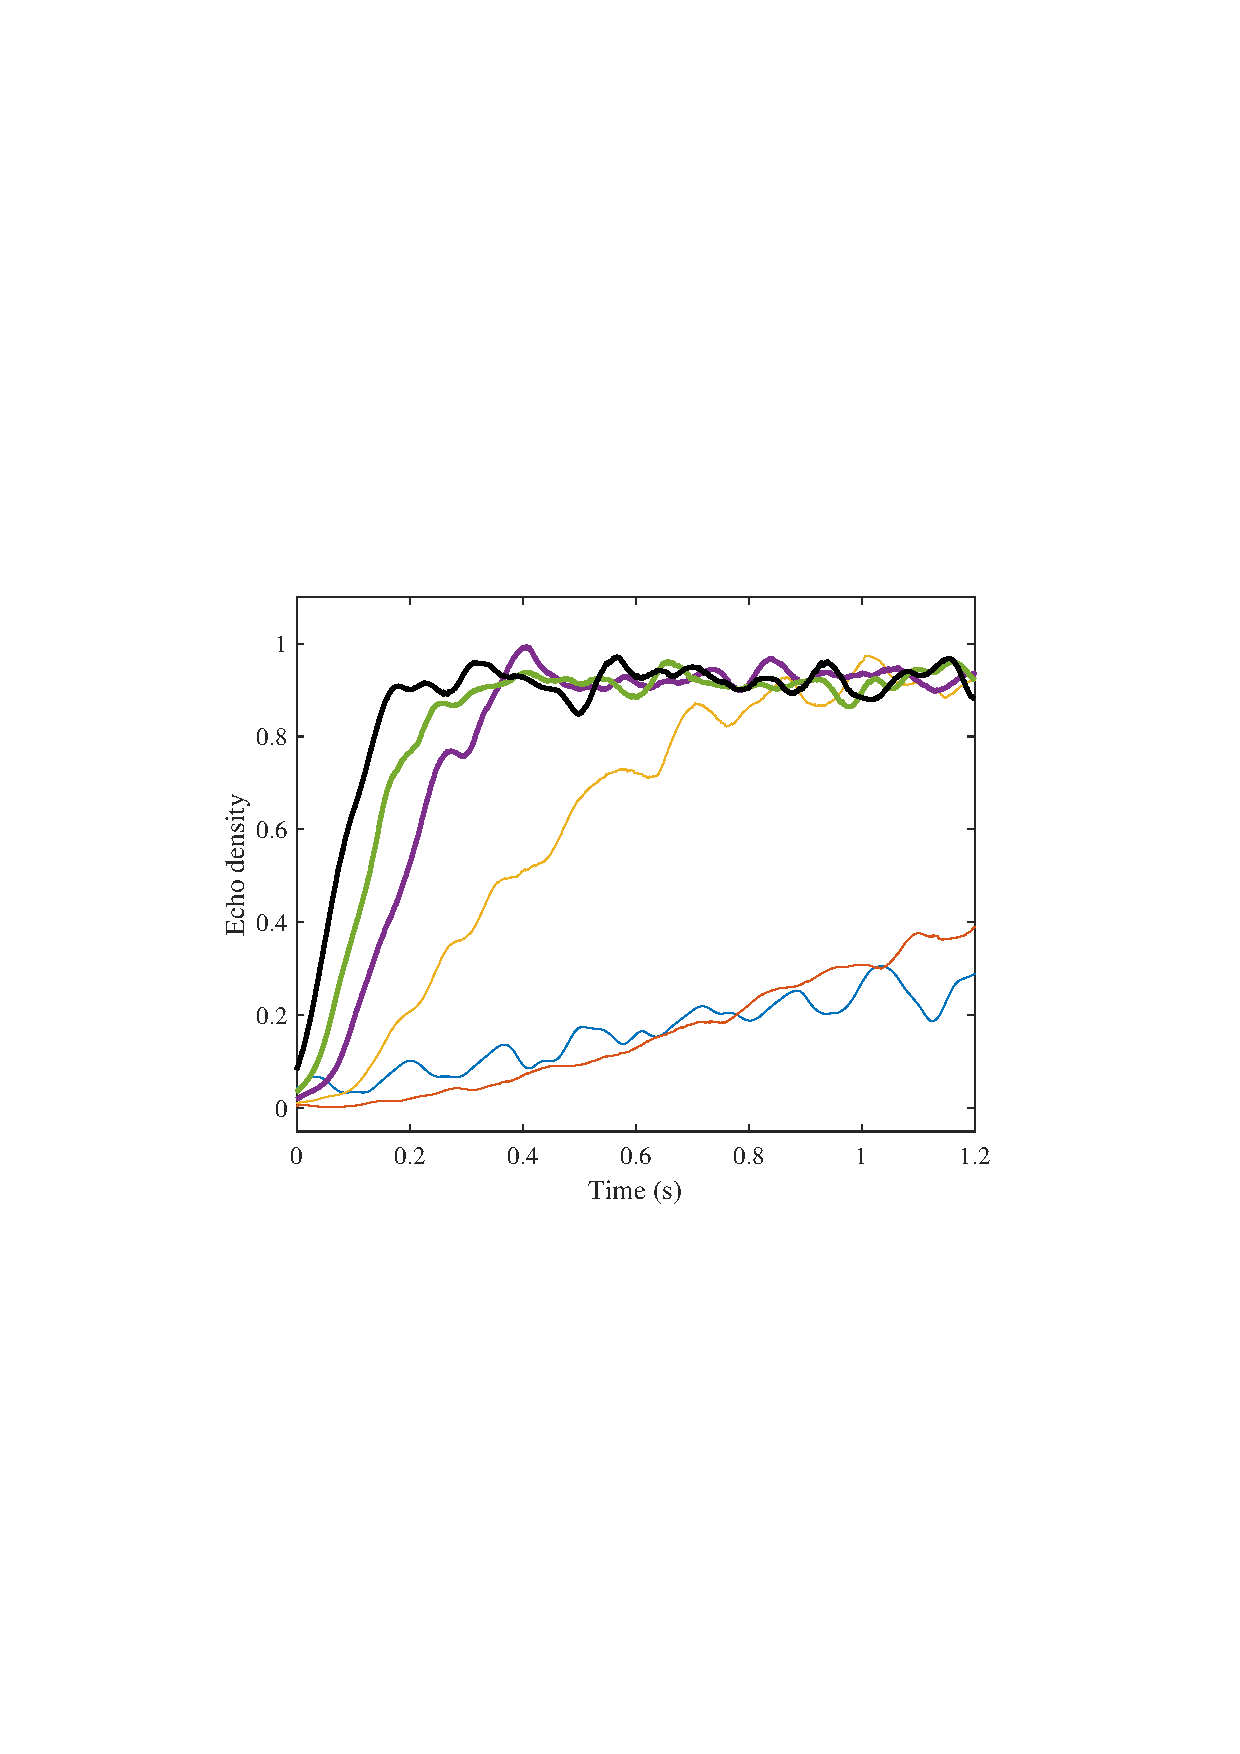
\includegraphics[trim=3.8cm 9.2cm 4.5cm 10cm, width=0.44\textwidth]{Figures/echoRand.pdf}}} \hfill
    \caption{\textit{Normalized echo densities for four types of feedback matrices and different FDN orders.}}
    \label{fig:echo}
\end{figure*}

\subsection{CPU Usage}
The CPU usage for all FDN orders for three different plugin-states -- unfixed coefficients plotting the IR, unfixed coefficients plotting the EQ and fixed coefficients (plotting and recalculation of filter coefficients disabled) -- can be seen in Table~\ref{tab:CPU}. The measurements have been done using a MacBook Pro with a 2.2\,GHz Intel i7 processor using \textit{Xcode}'s time profiler~\cite{Xcode}.

\begin{table}[h]
    \caption{\textit{CPU usage for all FDN orders in the cases of unfixed (plotting IR and EQ) and fixed coefficients.}}
    \centering
    \begin{tabular}{|c|c|c|c|}
    \hline
      FDN & \multicolumn{3}{|c|}{CPU usage (\%)} \\\cline{2-4}
      Order & unfixed (IR) & unfixed (EQ) & fixed \\
       \hline
       2 & 18.4 & 11.0 & 3.1\\
       4 & 19.8 & 12.0 & 5.4 \\
       8 & 22.7 & 15.2 & 7.9 \\
       16 & 28.6 & 22.2 & 13.3\\
       32 & 46.1 & 40.2 & 30.4\\
       64 & 110.5 & 100.1 & 92.5\\
         \hline
    \end{tabular}
    \label{tab:CPU}
\end{table}

\noindent For all plugin-states the CPU usage increases exponentially with the FDN order. Furthermore, fixing the coefficients and thus disabling the plotting and filter-coefficient calculation greatly decreases the plugin's CPU usage. Compared to the unfixed EQ case an additional \texttildelow8.0\% is added to the CPU usage. When plotting the IR versus the EQ, an additional \texttildelow7.5\% is added to the usage. This value, however, depends on the average reverb time used. Here, the \textit{Concert hall} preset was used which requires calculating 2.5\,s of sound for the IR plot. With a higher average slider value and thus a longer IR to be calculated and plotted, the CPU usage also increases.

As said in Sec.~\ref{subsubsec:feedbackMatrix} the smallest usable FDN order is 16. The results show that using this order or even 32 are unlikely to cause auditory drop-outs when used, especially when the coefficients are fixed.

\section{Conclusions}\label{sec:conclusion}

The present study introduces the FDN-based artificial reverberation synthesis plugin. The implementation allows controlling the decay characteristics of the sound in ten octave bands in real time%using three different modes
, and plots the corresponding RT curve, attenuation filter's magnitude and IR. %The plugin enables altering the gain of the input sound as well as the dry/wet mix. 
Additionally, the users can explore different setups of the FDN by changing the type and size of the feedback matrix, and the lengths and distribution of the delay lines. 

The experiments with the delay-line lengths and distribution suggest that those parameters should always be used in a balanced way, which suits the target reverberation. A wrong choice of the range may result in excess computation without a proportional increase in echo density. Using very short delay lines make the system more likely to become unstable. Choosing the lengths over narrow range results in low-quality sound, which diffuses slowly. Additionally, picking the right distribution is important as well. Using uniform distribution makes the overlaps of output samples inevitable. 

The ability to choose among different FDN orders shows that the lowest useful order for high-quality sound processing is 16, as it provides fast enough echo density build-up to obtain smooth reverberation without audible artifacts. Shifting between feedback matrix types proves that the identity matrix, even though it is lossless, should not be used in such applications, since the produced sound is fluttery. It also shows that in the case of the Householder matrix, implementation affects the reverberation. The construction of the 16-order Householder matrix through a recursive embedding results in the echo density reaching saturation faster and remaining more stable than when the implementation using the identity matrix is used.

\section{Acknowledgments}
This work was initialized, when Karolina Prawda made a Short-Term Scientific Mission to the Aalborg University Copenhagen on October 28 -- November 15, 2019. 

%\newpage
%\nocite{*}
\bibliographystyle{IEEEbib}
\bibliography{DAFx20_tmpl} % requires file DAFx20_tmpl.bib



\end{document}
